\documentclass[aspectratio=169]{beamer}

\usepackage[UTF8,fontset=none]{ctex}
\usepackage{fontspec}
\usepackage{graphicx}
\usepackage{booktabs}
\usepackage{amsmath, amssymb}
\usepackage{multicol}
\usepackage{array}
\usepackage{tabularx}
\usepackage{adjustbox}
\usepackage{tikz}
\usetikzlibrary{arrows.meta, shapes.geometric, positioning, calc, fit}
\usepackage{csquotes}
\usepackage{colortbl}       % \rowcolor in tables
\usepackage{listings}       % code listings
\usepackage{ccicons}    % Creative Commons icons

% listings global style
\lstset{
  basicstyle   = \ttfamily\scriptsize,
  keywordstyle = \color{blue!80!black}\bfseries,
  commentstyle = \color{gray}\itshape,
  stringstyle  = \color{teal},
  numbers      = left,
  numberstyle  = \tiny\color{gray},
  numbersep    = 6pt,
  frame        = single,
  rulecolor    = \color{gray!40},
  breaklines   = true,
  tabsize      = 2,
  showstringspaces = false,
}
\usepackage{hyperref}
\usepackage{appendixnumberbeamer}

\newcolumntype{Y}{>{\centering\arraybackslash}X}
\graphicspath{{figures/}{figures/paper/}}

% Stable local font root. This path is intentionally absolute because the
% font repository is kept in a fixed location outside the template project.
\newcommand{\FontRoot}{/Users/eamonsuen/Documents/GitHub/latex-chinese-fonts}

% English fonts
\setmainfont{TimesNewRoman.ttf}[
  Path = \FontRoot/english/Serif/,
  BoldFont = TimesNewRomanBold.ttf,
  ItalicFont = TimesNewRomanItalic.ttf,
  BoldItalicFont = TimesNewRomanBoldItalic.ttf
]
\setsansfont{Helvetica.ttf}[
  Path = \FontRoot/english/Sans/,
  BoldFont = HelveticaBold.ttf,
  ItalicFont = HelveticaOblique.ttf,
  BoldItalicFont = HelveticaBoldOblique.ttf
]
\setmonofont{Courier.ttf}[
  Path = \FontRoot/english/Mono/,
  BoldFont = CourierBold.ttf,
  ItalicFont = CourierOblique.ttf,
  BoldItalicFont = CourierBoldOblique.ttf
]

% Chinese fonts
\setCJKmainfont{FangSong.ttf}[
  Path = \FontRoot/chinese/仿宋体/,
  AutoFakeBold = true,
  AutoFakeSlant = true
]
\setCJKsansfont{STHeiti.ttf}[
  Path = \FontRoot/chinese/黑体/,
  AutoFakeBold = true,
  AutoFakeSlant = true
]
\setCJKmonofont{SimHei.ttf}[
  Path = \FontRoot/chinese/黑体/,
  AutoFakeBold = true,
  AutoFakeSlant = true
]

% Optional per-project override examples.
% \setmainfont{YourSerifFont.ttf}[Path=fonts/serif/]
% \setsansfont{YourSansFont.ttf}[Path=fonts/sans/]
% \setmonofont{YourMonoFont.ttf}[Path=fonts/mono/]

\usefonttheme{professionalfonts}
\usefonttheme{serif}
\usetheme{default}
\usecolortheme{default}
\useoutertheme{infolines}
\setbeamertemplate{navigation symbols}{}
\setbeamertemplate{caption}[numbered]

\title{数字化转型的投资结构优化效应}
\subtitle{第五届香樟数字经济论坛}
\author[王倩、孙翊铭]{王倩\inst{1,2} \and 孙翊铭\inst{2}\\[0.35em]{\small 汇报人：孙翊铭}}
\institute[吉林大学]{\inst{1}吉林大学国有经济研究中心 \and \inst{2}吉林大学经济学院\\ \texttt{sunym25@mails.jlu.edu.cn}}
\date{2026年5月10日 · 长春}
\hypersetup{
  pdftitle={数字化转型的投资结构优化效应},
  pdfauthor={王倩, 孙翊铭}
}

% Keep a single opening outline for a 20-minute conference talk.

\begin{document}

\begin{frame}
  \titlepage
\end{frame}

\begin{frame}{Outline}
  \begin{multicols}{2}
    \tableofcontents
  \end{multicols}
\end{frame}

\section{研究问题}

\begin{frame}{开场}
  各位老师、各位同学，大家好。

  \vspace{0.6em}
  我今天汇报的题目是《数字化转型的投资结构优化效应》，这是我和我的导师王倩教授合作完成的一篇文章。

  \vspace{0.8em}
  接下来的汇报，我打算沿着这样一个思路展开：
  \begin{enumerate}
    \item 先跟大家聊聊我们为什么要关心这个问题；
    \item 然后介绍我们是怎么用模型把故事讲清楚的；
    \item 再看看数据上能不能找到支持这个故事的证据；
    \item 最后讨论这些发现意味着什么。
  \end{enumerate}
\end{frame}

\begin{frame}{一个持续了近三十年的宏观趋势}
  \begin{figure}
    \centering
    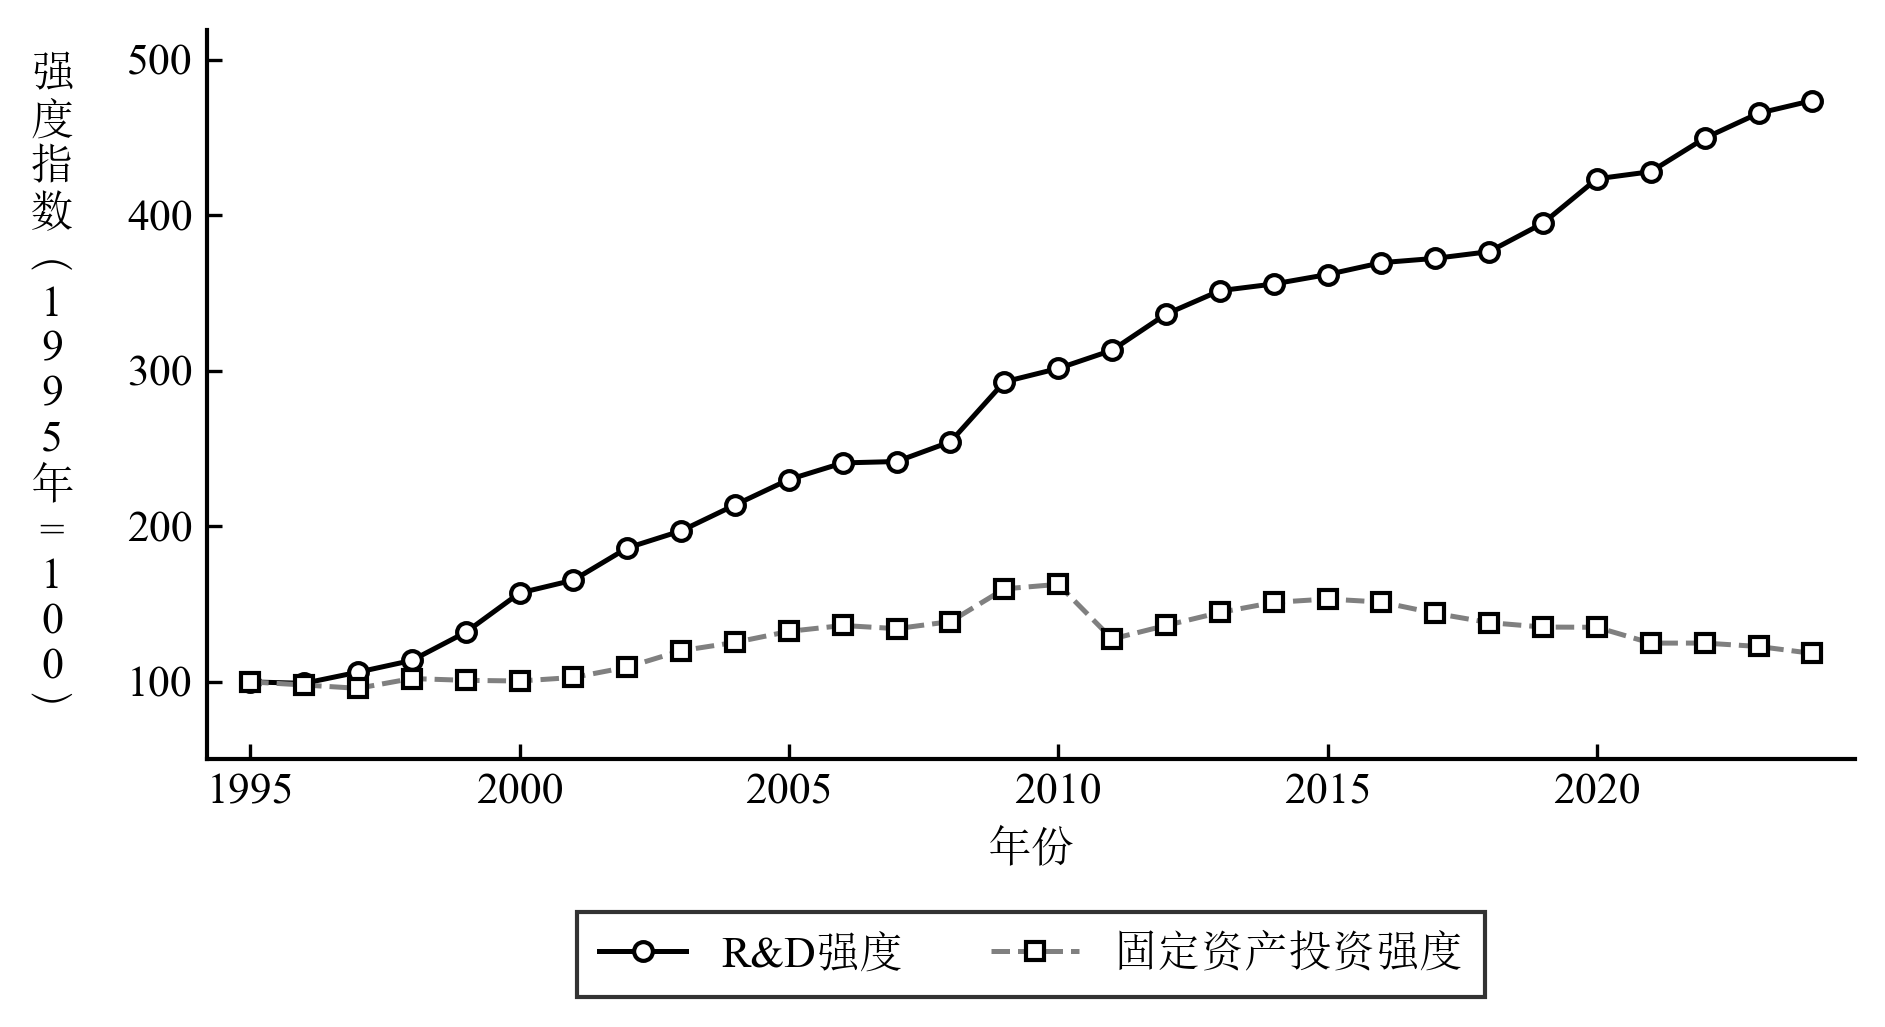
\includegraphics[width=0.78\linewidth,height=0.62\textheight,keepaspectratio]{figures/paper/macro-rd-fai-1995.png}
    \caption{1995--2023 年研发支出指数与固定资产投资指数（1995 年=100）}
  \end{figure}
\end{frame}

\begin{frame}{这个图告诉了我们什么？}
  大家看一下这张图，两条线的走势一目了然：

  \begin{itemize}
    \item 1995 年的时候，中国研发经费占全社会固定资产投资的比重，\textbf{不到 2\%}；
    \item 到了 2023 年，这个数字已经超过了 \textbf{10\%}；
    \item 而且大家注意，两条线的分化在 2008 年金融危机之后明显加速了。
  \end{itemize}

  \vspace{0.5em}
  换句话说，中国企业的投资正在发生一个结构性的转变：\textbf{盖厂房、买设备的钱相对变少了，搞研发、做创新的钱相对变多了}。
\end{frame}

\begin{frame}{已有解释，以及它们没有回答的问题}
  怎么理解这个趋势？已有的研究大致给了两种说法：

  \begin{itemize}
    \item 一种比较悲观：实物投资收缩说明企业信心不足、总需求疲软，担心是不是资产负债表衰退；
    \item 另一种相对乐观：软件、数据、专利这些无形资产正在替代传统的机器设备。
  \end{itemize}

  \vspace{0.5em}
  但我总觉得这两种解释都缺了一环——

  \begin{cautionbox}{一个绕不过去的问题}
    在融资难、融资贵普遍存在的现实下，企业为什么能\emph{一边减少实物投资、一边扩大研发投入}？这种"此消彼长"如果不是简单的规模收缩，那背后的驱动力是什么？
  \end{cautionbox}
\end{frame}

\begin{frame}{为什么说这是一个可识别的问题？}
  \begin{itemize}
    \item 我们注意到，这个投资结构转变的时间窗口，恰好与中国产业数字化政策的推进节奏高度吻合。
    \item 尤其是\emph{两化融合管理体系贯标}——这是一个企业层面的数字化治理能力认证，截至 2025 年 4 月，贯标企业已经超过 \textbf{7.4 万家}。
    \item 对我们做实证的人来说，这个制度设计提供了一个很好的识别条件：\emph{认证通过日可观测，试点分批推进}——天然就是一个交叠 DID 的设定。
  \end{itemize}

  \begin{findingbox}{所以本文要回答的核心问题是}
    数字化通过什么样的渠道，让原本受融资约束压制的企业，把资金从低效的实物囤积转向了研发和创新？
  \end{findingbox}
\end{frame}

\begin{frame}{切入的角度：从融资契约看问题}
  我们的分析角度可能和已有文献不太一样——我们是从\emph{融资契约是怎么写的}这个角度切入的。

  \begin{itemize}
    \item 在金融市场不完美的情况下，企业借钱很大程度上要靠资产做抵押。
    \item 这就导致实物资产（厂房、设备、土地）在企业账上\emph{同时承担两种角色}：既是干活的工具，也是借钱的凭据。
    \item 当"借钱的凭据"这个角色压倒"干活的工具"时，企业就会把实物资本推到超出生产需要的水平——我们管这叫\emph{抵押囤积}。
  \end{itemize}
\end{frame}

\begin{frame}{数字化的关键作用：让信息替代抵押}
  那数字化在其中扮演什么角色？这里需要引入近年文献的一个重要发现：

  \begin{itemize}
    \item Lian 和 Ma（2021）发现，美国大约 \textbf{80\%} 的企业债务其实不是靠资产抵押，而是基于经营现金流；
    \item 万晓莉等（2025）进一步记录了中国企业的融资模式也在从抵押物导向转向现金流导向。
  \end{itemize}

  \vspace{0.4em}
  这意味着什么？意味着企业借钱其实有两条路——\emph{资产抵押}和\emph{现金流抵押}。

  \begin{findingbox}{数字化的角色：信息替代抵押}
    数字化让企业的经营活动变得更加标准化、可记录、可验证。当银行能看到、能相信企业的经营数据时，现金流信息就开始替代实物抵押品发挥作用。这时候，那些原本为了借钱而多囤的设备厂房，就可以慢慢退出了。
  \end{findingbox}
\end{frame}

\begin{frame}{本文的三个边际贡献}
  \begin{enumerate}
    \item \textbf{理论上}：我们把资产抵押和现金流抵押同时放进一个两期投融资模型，推导出一个关于实物资本边际收益的\emph{门槛命题}——这解释了为什么同样面临数字化，不同企业的投资调整方向可能截然不同。
    \item \textbf{识别上}：利用两化融合贯标的分批推进构造准自然实验，并吸收了 Nagengast 和 Yotov（2025）、Bertolotti（2026）处理预期效应的最新方法。
    \item \textbf{机制上}：沿着\emph{信息替代抵押 $\rightarrow$ 抵押囤积出清 $\rightarrow$ 配置效率改善}这条逻辑链，给出了层层递进的经验证据。
  \end{enumerate}
\end{frame}

\section{制度背景与机制}

\begin{frame}{制度背景：两化融合贯标}
  \begin{itemize}
    \item 两化融合：以信息化推动工业化、以工业化促进信息化。
    \item 管理体系贯标将数字化从零散技术改造转化为可复制、可审计、可持续改进的组织流程。
    \item 截至2025年4月，贯彻两化融合管理体系标准的企业超过7.4万家。
    \item 贯标严格依据国家统一标准，由独立第三方机构现场审查与分级认证。
    \item 地区与年份维度上的分批推进，为交叠双重差分提供政策环境。
  \end{itemize}
\end{frame}

\begin{frame}{政策推进：财政激励与试点示范}
  \begin{figure}
    \centering
    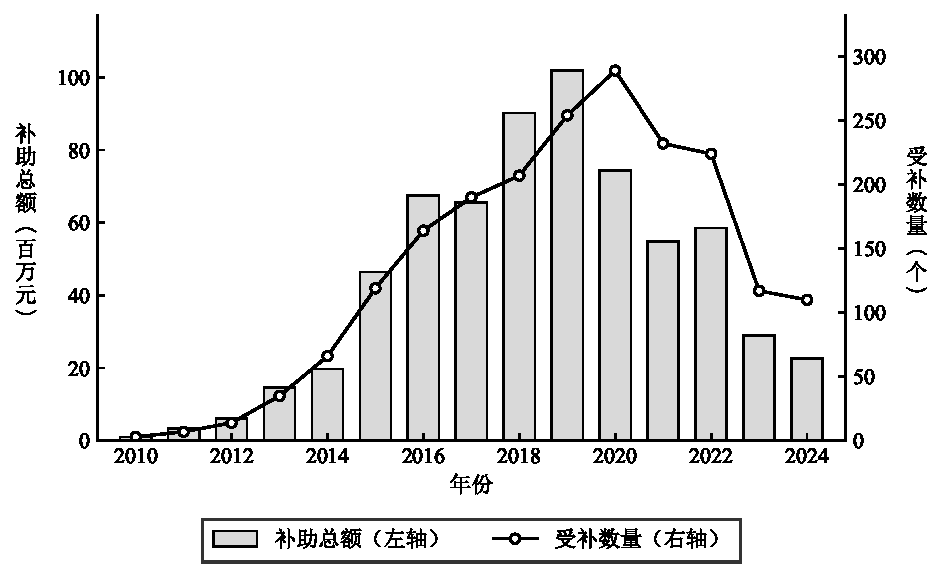
\includegraphics[width=0.82\linewidth,height=0.62\textheight,keepaspectratio]{Subsidy_Trend.pdf}
    \caption{上市公司获得的“两化融合”相关政府补助}
  \end{figure}
\end{frame}

\begin{frame}{宏观事实：固定投资与研发投入分化}
  \begin{figure}
    \centering
    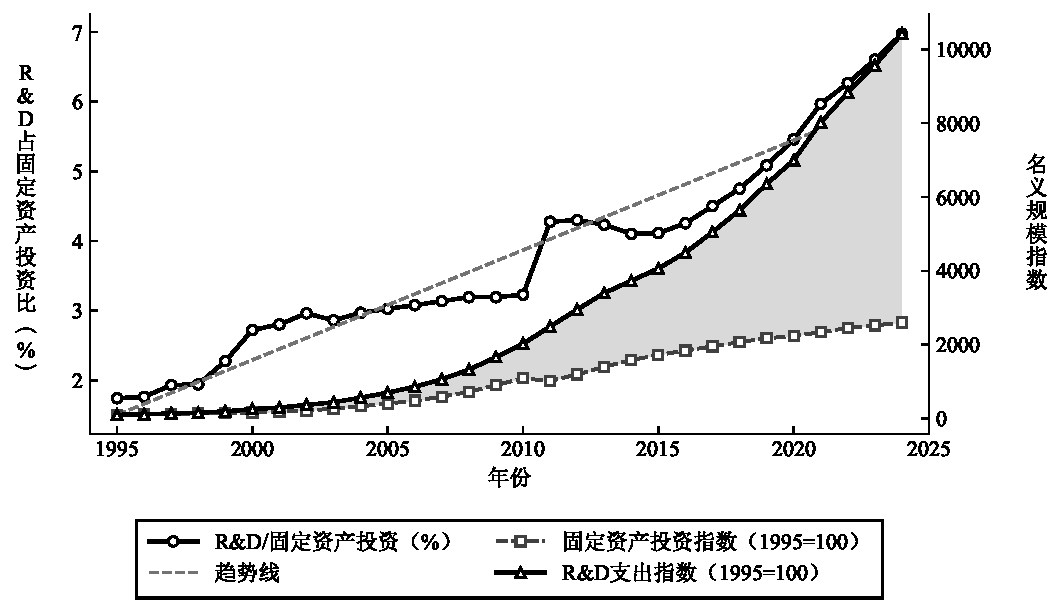
\includegraphics[width=0.82\linewidth,height=0.62\textheight,keepaspectratio]{Macro_RDShare_LeftAxis_Index_RightAxis_1995base_BW.pdf}
    \caption{固定投资与研发投入的相对变化}
  \end{figure}
\end{frame}

\begin{frame}{微观事实：实物投资与研发投入}
  \begin{figure}
    \centering
    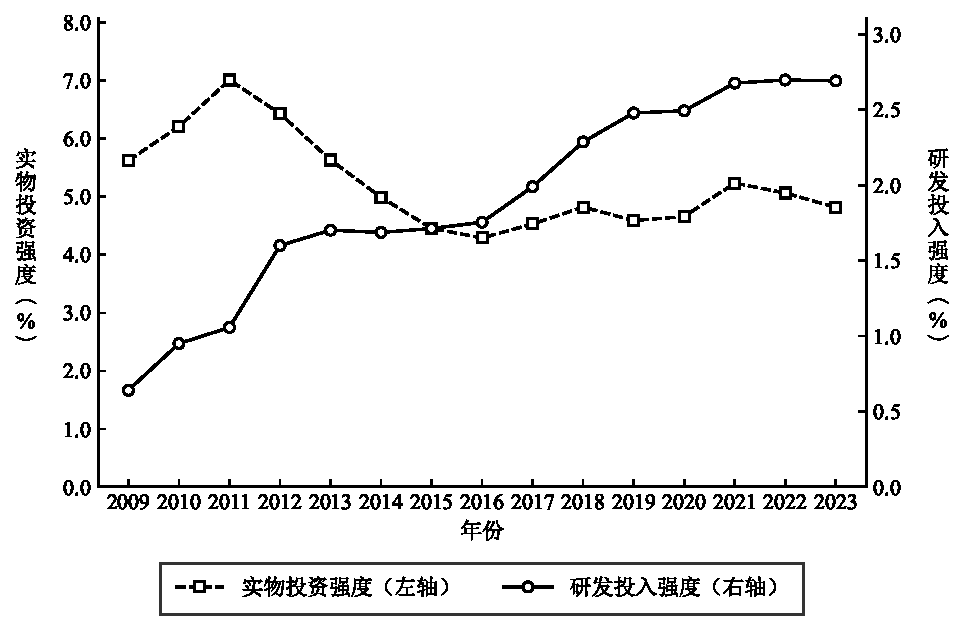
\includegraphics[width=0.82\linewidth,height=0.62\textheight,keepaspectratio]{Micro_Investment_Structure_Scissors.pdf}
    \caption{上市企业投资结构的剪刀差}
  \end{figure}
\end{frame}

\begin{frame}{机制：抵押品替代与投资结构}
  \begin{columns}[T]
    \column{0.48\textwidth}
      \textbf{传统约束}
      \begin{itemize}
        \item 外部融资依赖可抵押资产。
        \item 实物资本兼具生产功能与抵押功能。
        \item 研发更难估值、清算与抵押。
      \end{itemize}
    \column{0.48\textwidth}
      \textbf{数字化冲击}
      \begin{itemize}
        \item 数据留痕改善信息可验证性。
        \item 经营现金流更容易契约化。
        \item 融资契约减少对实物抵押的依赖。
      \end{itemize}
  \end{columns}
  \vspace{0.7em}
  \begin{center}
    \large 预测：抵押囤积型企业收缩 CapEX，研发投入无条件扩张
  \end{center}
\end{frame}

\begin{frame}{理论预测：门槛命题}
  \begin{itemize}
    \item 企业同时面临资产抵押与现金流抵押双重摩擦。
    \item 数字化缓解融资约束后，有形资本调整方向取决于企业抵押能力是否超过临界水平。
    \item 抵押能力低于阈值：原本融资不足，约束缓解后增加有形资本投入。
    \item 抵押能力高于阈值：原本为融资囤积实物资产，约束缓解后收缩冗余产能。
    \item 研发投入扩张不依赖于有形资本调整方向，是本文实证预测的核心不对称性。
  \end{itemize}
\end{frame}

\section{研究设计}

\begin{frame}{数据与样本}
  \begin{itemize}
    \item 样本：2009--2023 年 A 股上市公司。
    \item 处理变量：企业获得两化融合贯标试点或认证后取 1。
    \item 结果变量：
      \begin{itemize}
        \item CapEX1：购建固定资产、无形资产和其他长期资产支付的现金 / 总资产。
        \item RD1：研发支出 / 总资产。
        \item RD2 与研发投资作为替代研发投入指标。
      \end{itemize}
    \item 连续变量进行 1\% 和 99\% 分位缩尾，剔除金融类与异常样本。
  \end{itemize}
\end{frame}

\begin{frame}{基准模型}
  \begin{block}{交叠双重差分}
  \begin{align*}
    y_{it} = \alpha_i + \gamma_t + \beta D_{it}
    + \theta X_i \times f(t) + \varepsilon_{it}
  \end{align*}
  \end{block}
  \begin{itemize}
    \item $\alpha_i$：企业固定效应；$\gamma_t$：年份固定效应。
    \item $X_i \times f(t)$：基期企业特征与时间三次多项式交互，吸收事前禀赋导致的差异化趋势。
    \item 标准误聚类到企业层面。
  \end{itemize}
\end{frame}

\begin{frame}{处理时点：允许有限提前反应}
  \begin{itemize}
    \item 两化融合并非突发性冲击，贯标包含“实施--评估--认证”的过程。
    \item 企业可能在可观测认证节点之前已经开始对标改造与投入调整。
    \item 基准事件研究以认证完成节点为统一可观测事件时间。
    \item 同时通过事前趋势诊断和有限预期窗口设定，检验主结论对提前反应处理的敏感性。
  \end{itemize}
\end{frame}

\begin{frame}{无预期效应检验}
  \begin{columns}[T]
    \column{0.5\textwidth}
      \centering
      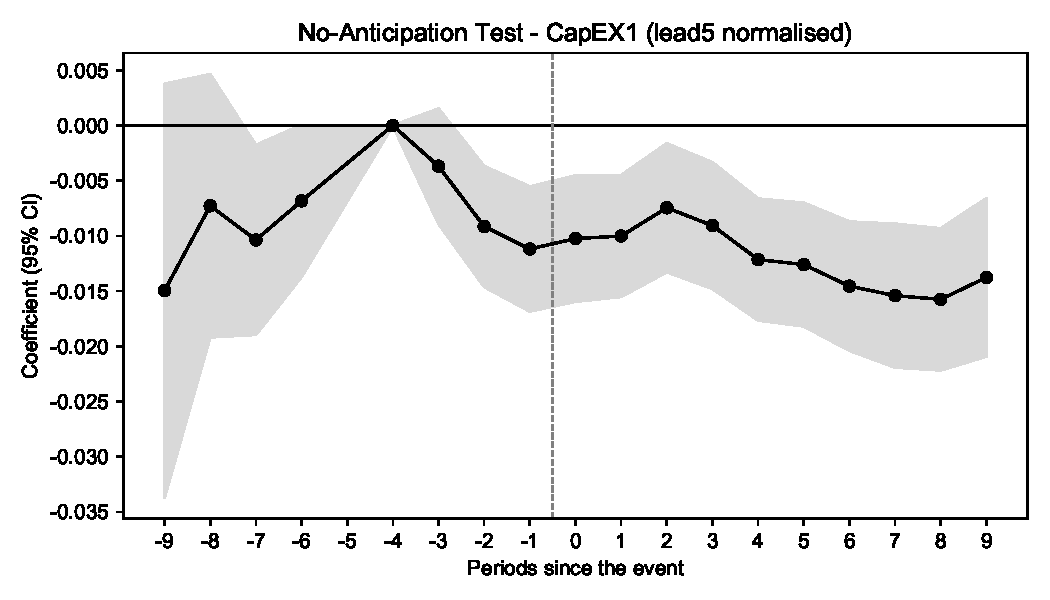
\includegraphics[width=\linewidth,height=0.62\textheight,keepaspectratio]{NoAnticipation_CapEX.pdf}
    \column{0.5\textwidth}
      \centering
      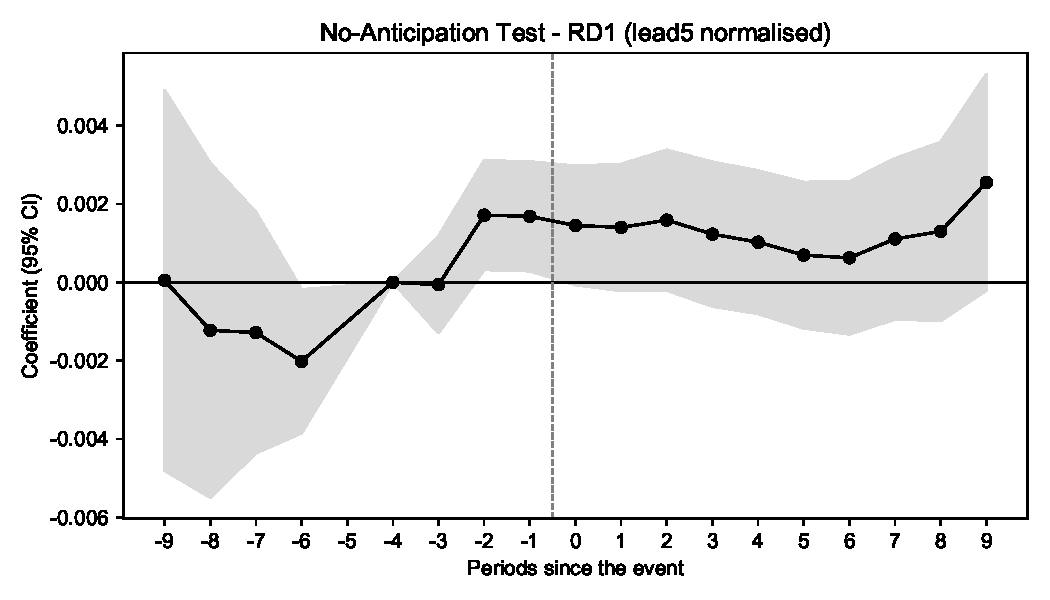
\includegraphics[width=\linewidth,height=0.62\textheight,keepaspectratio]{NoAnticipation_RD.pdf}
  \end{columns}
\end{frame}

\begin{frame}{识别假设与稳健性路径}
  \begin{itemize}
    \item 共同趋势：若未发生贯标冲击，处理组与对照组的投资结构应保持相似演进趋势。
    \item 进入年份检验：政策实施年份不应由处理前投资水平或趋势系统预测。
    \item 异质性稳健 DID：CSDID、DCDH、SA、BSJ、Stacked DID。
    \item 安慰剂检验：伪处理时点、随机处理组、混合随机化。
    \item 替代解释：供给侧去产能、金融去杠杆、房地产周期与投入产出网络溢出。
  \end{itemize}
\end{frame}

\section{实证证据}

\begin{frame}{样本与识别策略}
  好，现在来看数据。我们的样本是 2009--2023 年的 A 股上市公司。

  \vspace{0.4em}
  识别策略是交叠双重差分，核心设定是：
  \[
    Y_{it}=\alpha_i+\gamma_t+\beta D_{it}
    +\Gamma X_i \times f(t)+\varepsilon_{it}.
  \]

  \begin{itemize}
    \item $D_{it}$ 是企业 $i$ 在 $t$ 年是否已通过贯标认证；
    \item $\alpha_i$ 和 $\gamma_t$ 分别控制企业固定效应和年份固定效应；
    \item 识别来自于\emph{同一家企业贯标前后的投资结构变化}，同时由尚未贯标的企业提供对照。
  \end{itemize}

  \vspace{0.4em}
  $X_i\times f(t)$ 是事前特征与年份三次多项式的交乘——这么做的目的是在控制事前差异的同时，避免把政策后的变量当成坏控制。
\end{frame}

\begin{frame}{贯标企业的进入时间分布}
  \begin{figure}
    \centering
    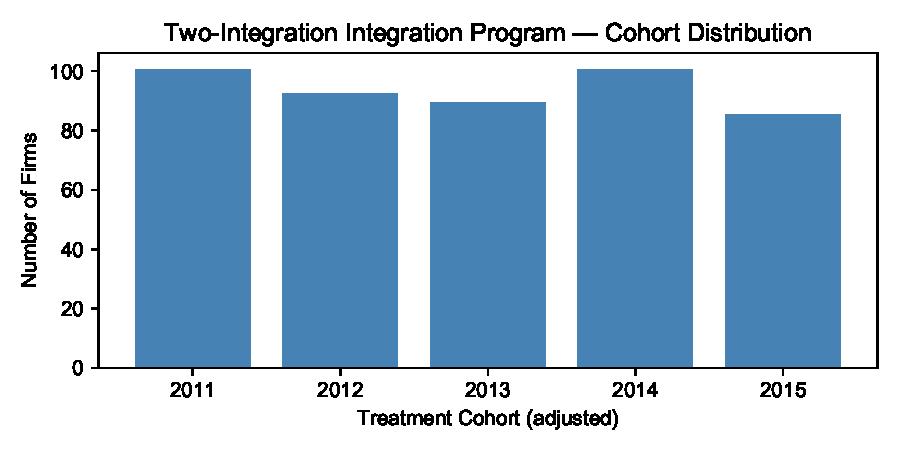
\includegraphics[width=0.65\linewidth,height=0.68\textheight,keepaspectratio]{figures/paper/Cohort_Distribution.pdf}
    \caption{各批次贯标企业的数量分布}
  \end{figure}
\end{frame}

\begin{frame}{为什么不能假设"无预期"？}
  前面提到过，两化融合不是突发冲击。如果忽略预期效应，事前系数就会被污染。

  \vspace{0.4em}
  我们的处理方式是：
  \begin{itemize}
    \item 把有效处理起点前移到认证通过日之前若干期；
    \item 用事前趋势诊断和有限预期窗口，把预期效应和实际处理效应分开。
  \end{itemize}

  \vspace{0.4em}
  具体来说，我们估计：
  \[
    Y_{it}=\alpha_i+\gamma_t
    +\sum_{l=-K_1}^{-2}\mu_lD_{it}^{l}
    +\sum_{l=0}^{K_2}\mu_lD_{it}^{l}
    +\Gamma X_i\times f(t)+\varepsilon_{it}.
  \]
\end{frame}

\begin{frame}{事件研究：预期被适当处理后}
  \begin{figure}
    \centering
    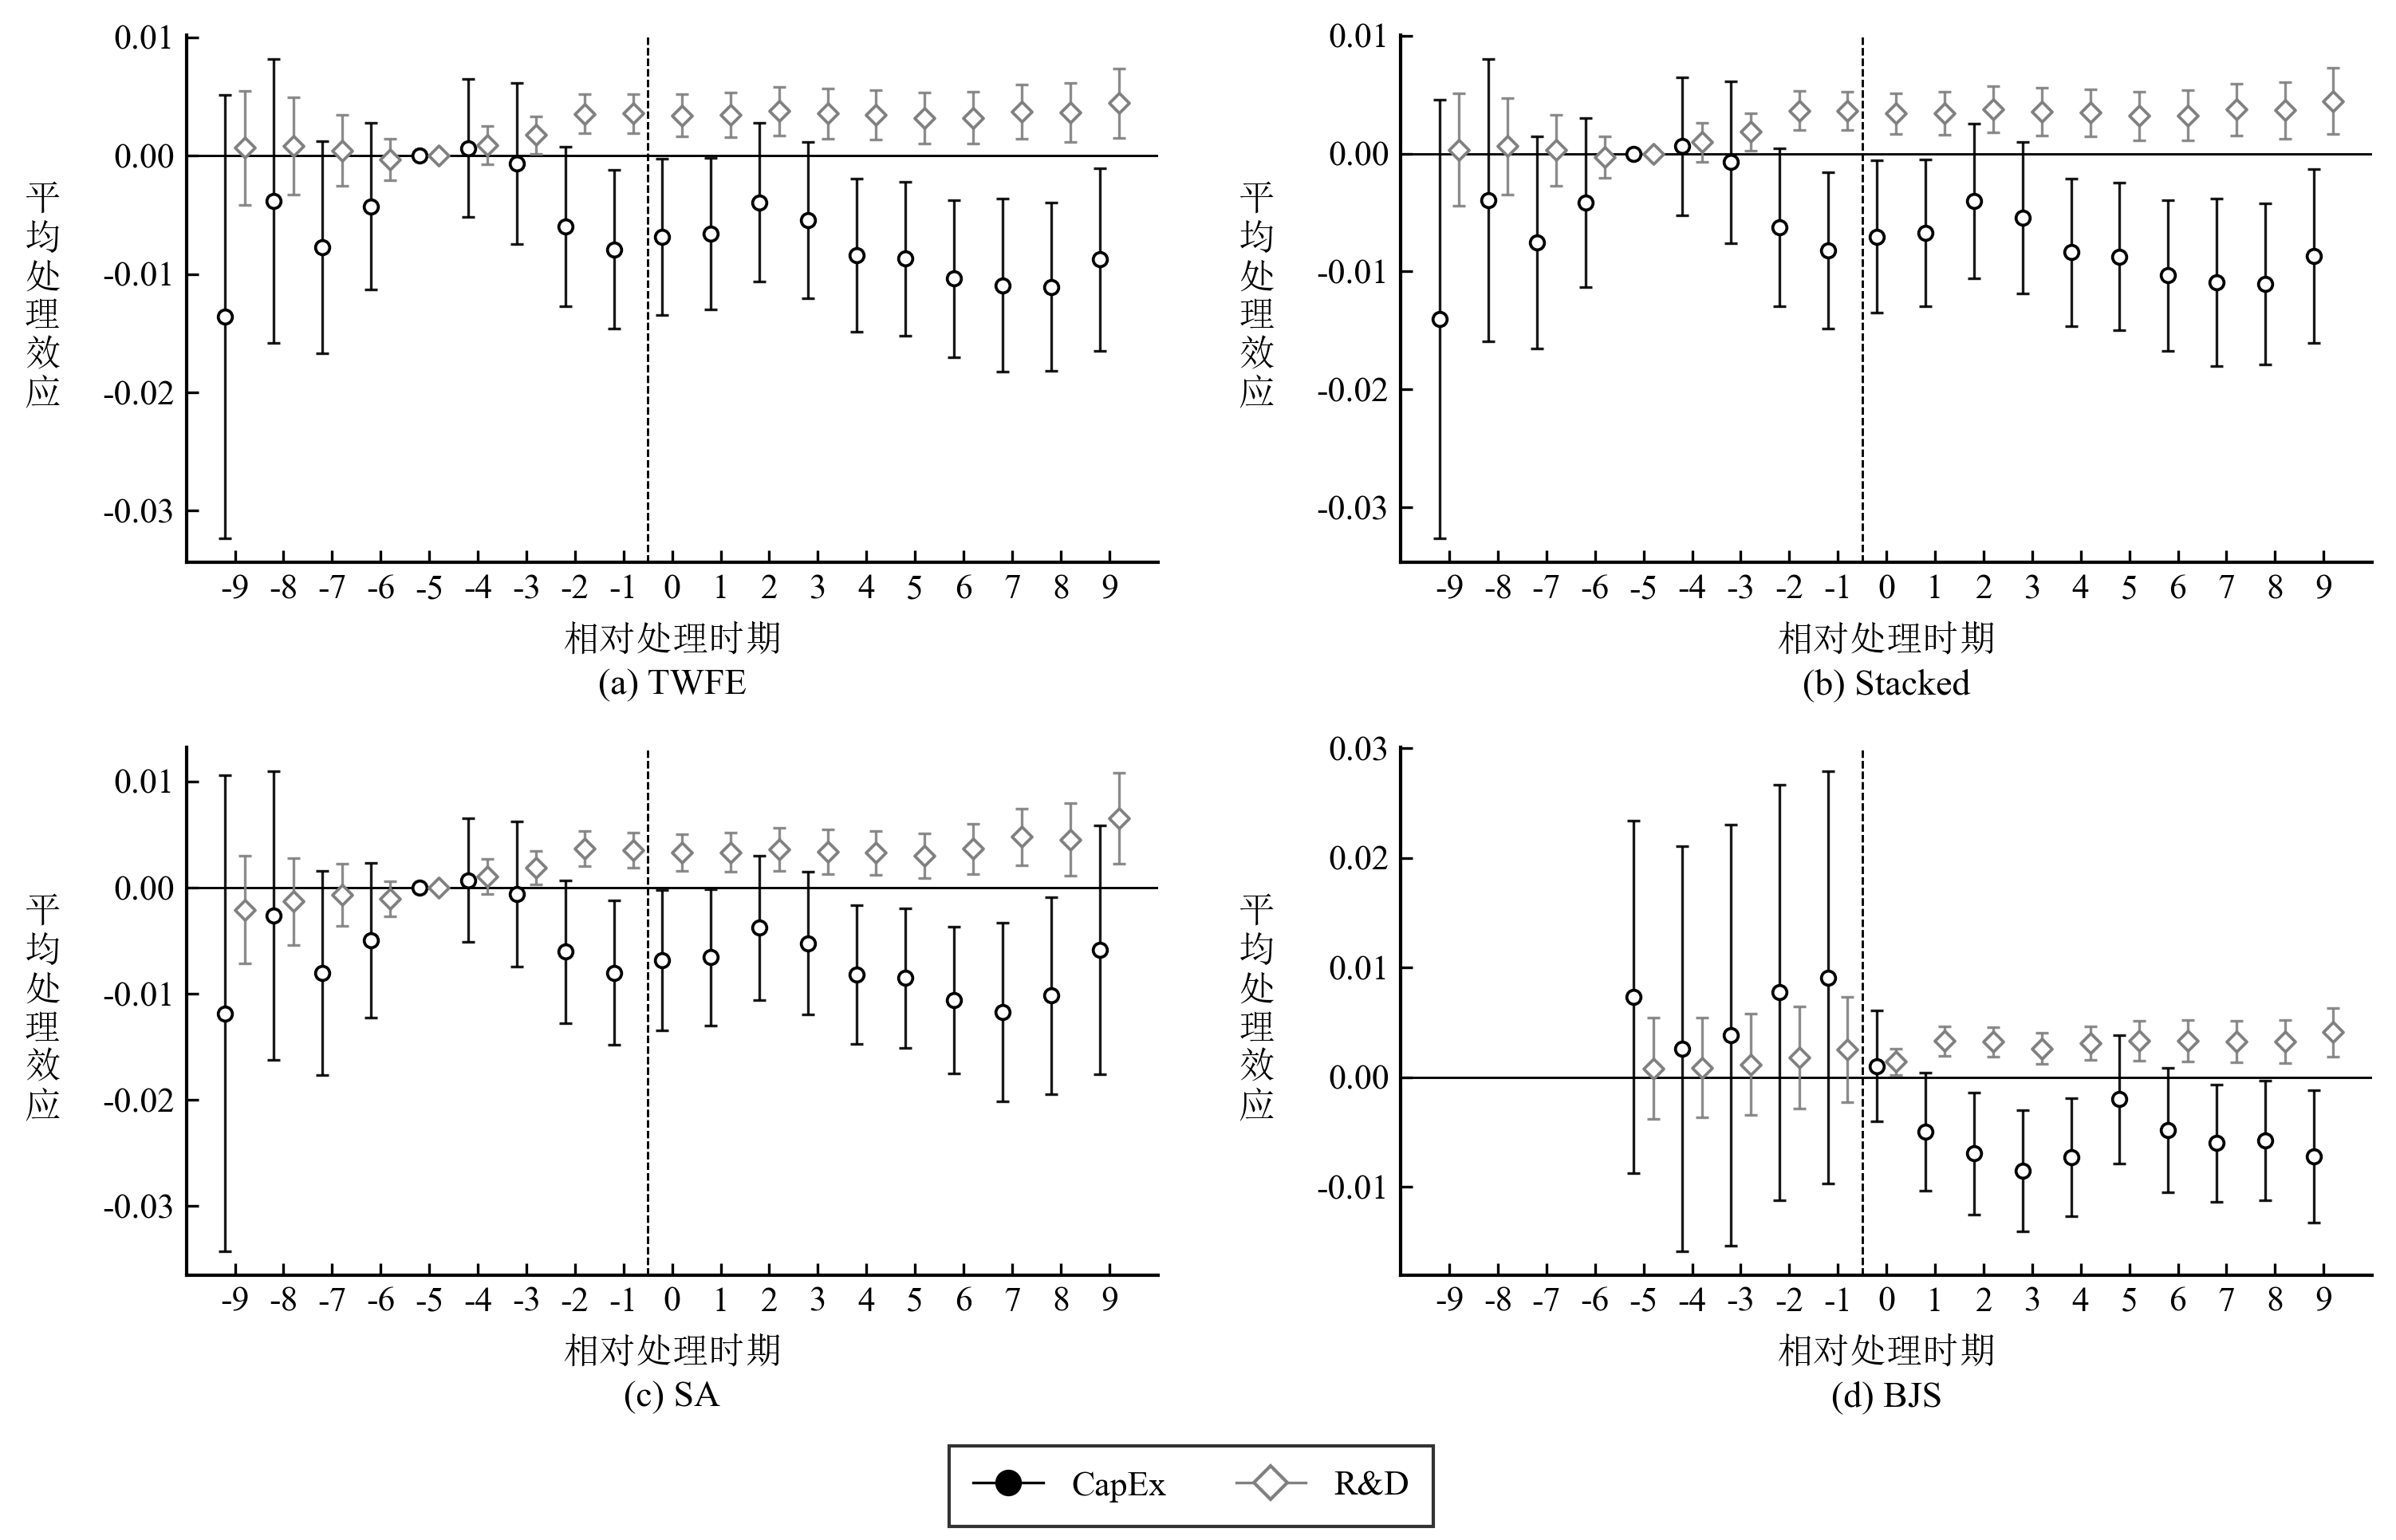
\includegraphics[width=0.86\linewidth,height=0.68\textheight,keepaspectratio]{figures/paper/anticipation-event-study.png}
    \caption{控制有限预期窗口后的事件研究：左为 CapEX，右为 R\&D}
  \end{figure}
\end{frame}

\begin{frame}{基准结果：一降一升}
  {\scriptsize
\begin{center}
\begin{tabular}{lcccc}
  \toprule
  变量 & (1) CapEX & (2) CapEX & (3) R\&D & (4) R\&D \\
  \midrule
  两化融合 & $-0.006^{**}$ & $-0.005^{**}$ & $0.003^{***}$ & $0.003^{***}$ \\
             & (0.002) & (0.002) & (0.001) & (0.001) \\
  控制变量 & 否 & 是 & 否 & 是 \\
  个体固定效应 & 是 & 是 & 是 & 是 \\
  时间固定效应 & 是 & 是 & 是 & 是 \\
  样本量 & 44,762 & 44,759 & 44,789 & 44,786 \\
  调整 $R^2$ & 0.493 & 0.496 & 0.819 & 0.820 \\
  \bottomrule
\end{tabular}
\end{center}
}


  \vspace{0.4em}
  \begin{findingbox}{经济含义}
    贯标后，企业实物投资水平相对于均值下降了约 \textbf{9.8\%}，而研发支出相对于均值上升了约 \textbf{14.3\%}。
  \end{findingbox}

  \vspace{0.3em}
  方向完全符合模型的第一个预测——实物投资降，研发投入升。
\end{frame}

\begin{frame}{这个"剪刀差"长什么样？}
  \begin{figure}
    \centering
    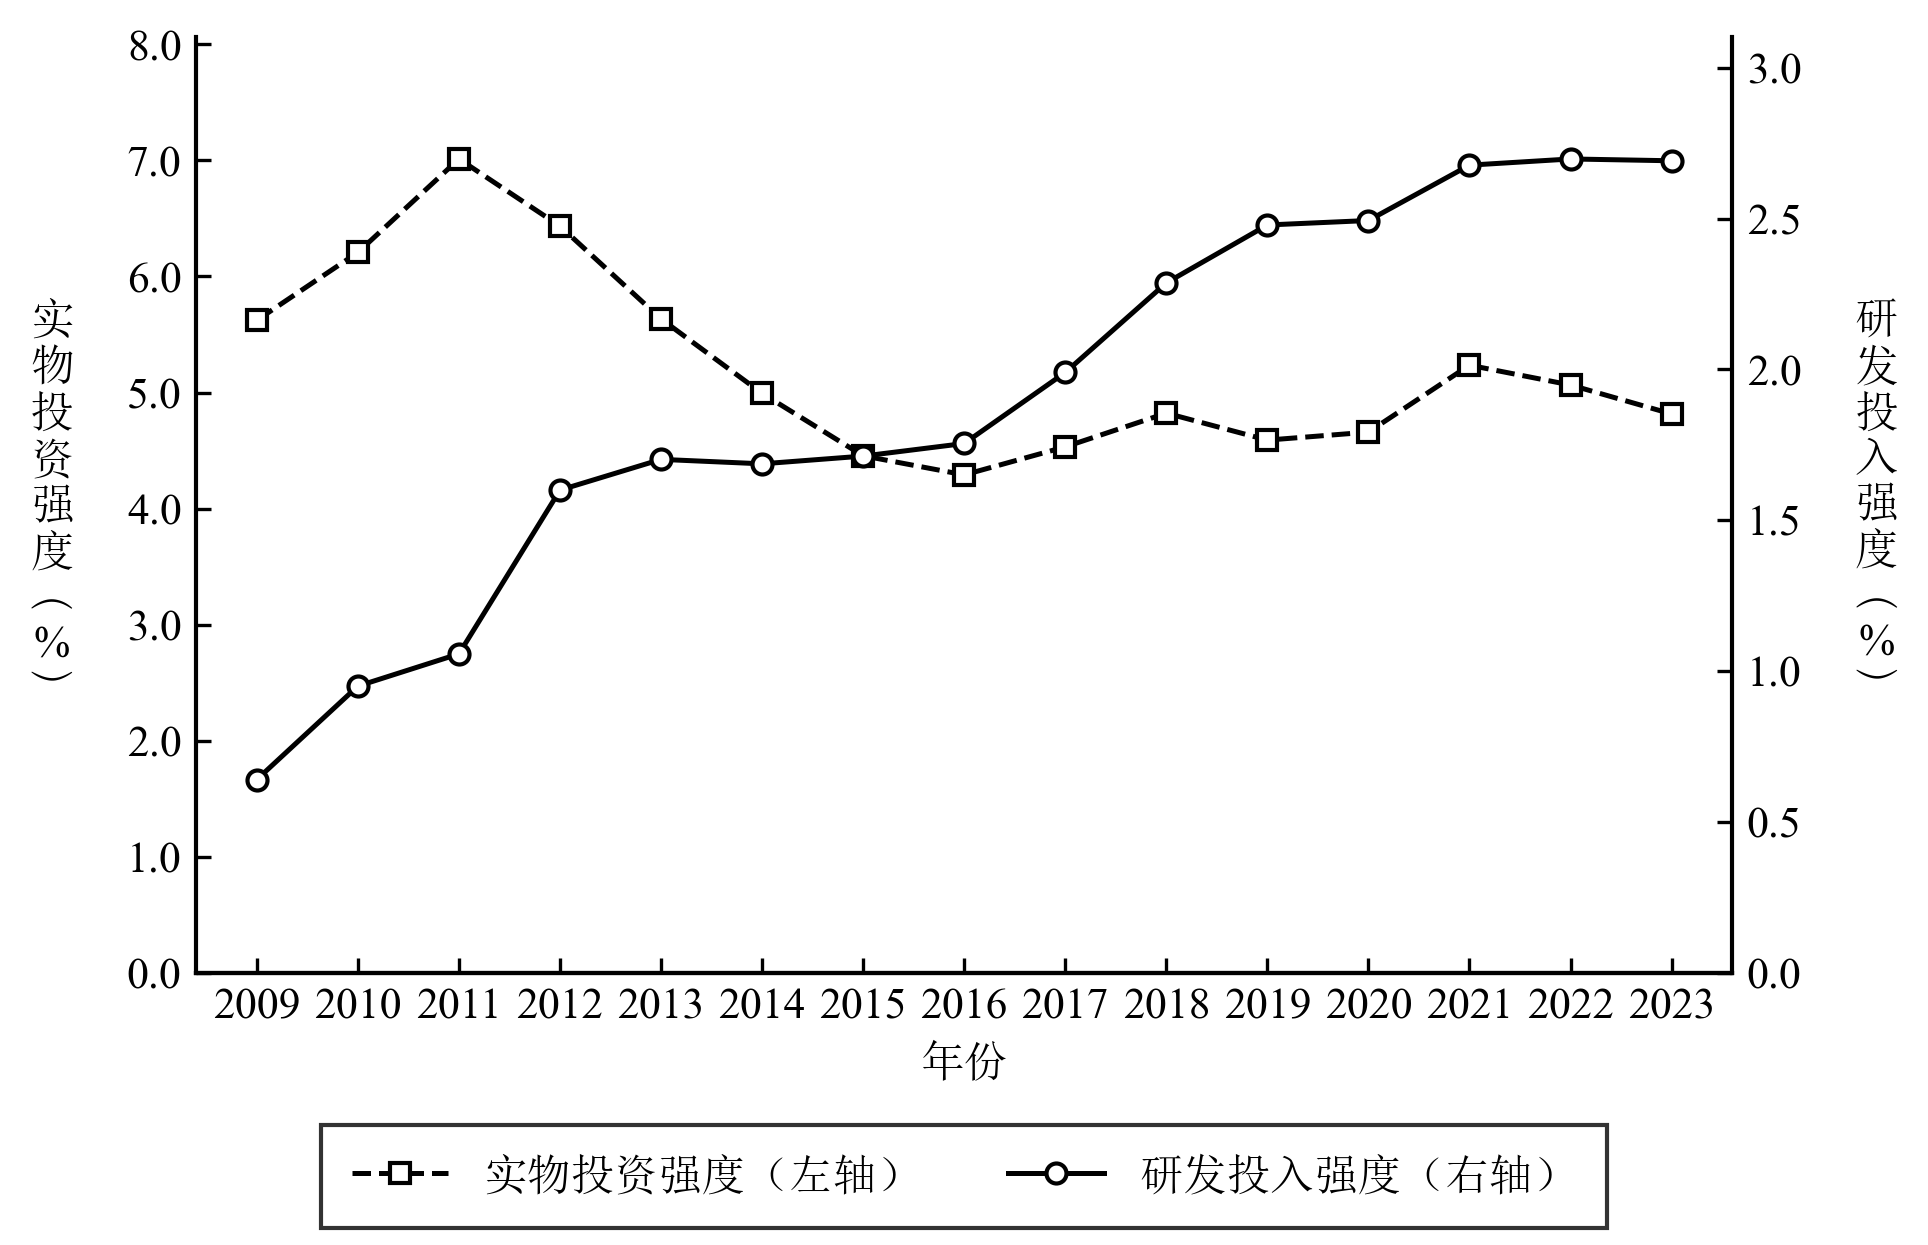
\includegraphics[width=0.78\linewidth,height=0.62\textheight,keepaspectratio]{figures/paper/micro-investment-structure.png}
    \caption{上市企业层面，实物投资与研发投入的分化趋势}
  \end{figure}
\end{frame}

\begin{frame}{稳健性：换估计量、换样本、换设定}
  基准结果稳不稳？我们做了以下检验：

  \begin{itemize}
    \item 使用 Sun--Abraham、Callaway--Sant'Anna、Borusyak--Jaravel--Spiess 等异质性稳健估计量，结论不变；
    \item PSM-DID、合成控制 DID、堆叠 DID 的结果一致；
    \item 控制投入产出网络溢出后，结论仍在。
  \end{itemize}

  \vspace{0.5em}
  我们还专门排除了几个竞争性解释：
  \begin{itemize}
    \item 控制供给侧去产能、金融去杠杆、房地产价格波动等宏观冲击后，CapEX 降、R\&D 升的结论没有变化。
  \end{itemize}
\end{frame}

\begin{frame}{稳健性：多估计量对比与安慰剂检验}
  \begin{figure}
    \centering
    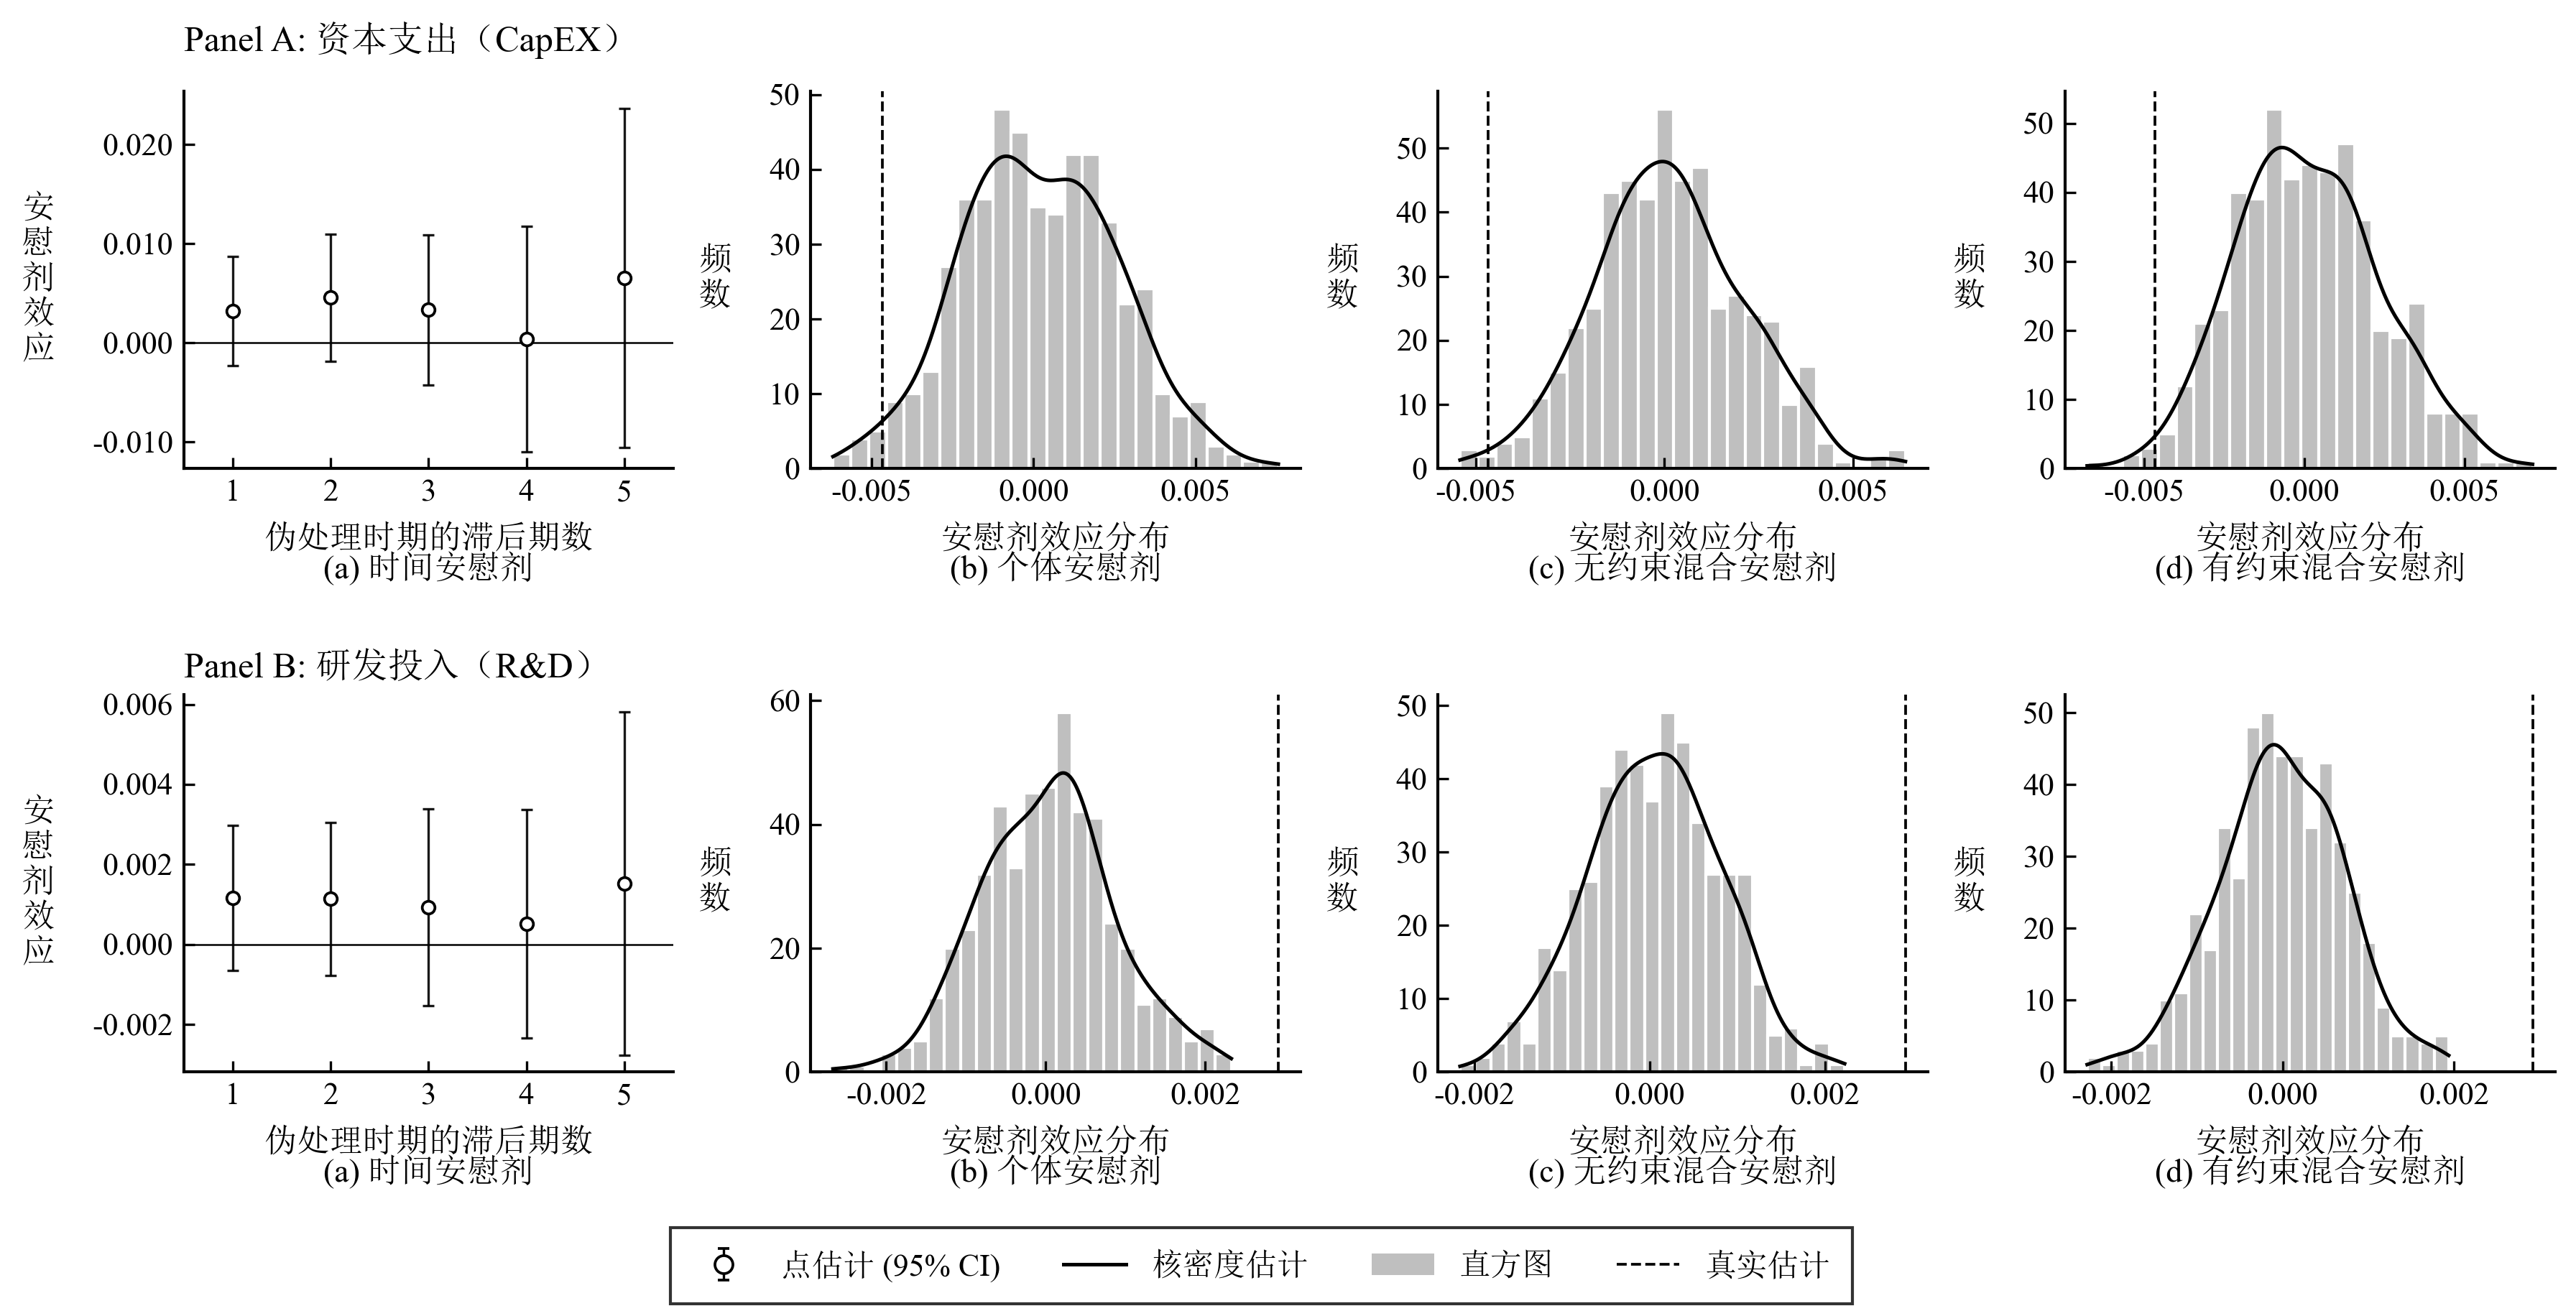
\includegraphics[width=0.8\linewidth,height=0.68\textheight,keepaspectratio]{figures/paper/placebo-tests.png}
    \caption{安慰剂检验与多种异质性稳健估计量的对比}
  \end{figure}
\end{frame}

\begin{frame}{机制一：怎么度量"抵押囤积"？}
  模型的第二个预测是：CapEX 收缩应该集中在那些事前囤积了大量超额资本的企业。

  \vspace{0.4em}
  怎么衡量"囤积"？我们构造了一个\emph{事前囤积楔子 PH}：
  \[
    \ln K_{it}
    =
    \beta_0+\beta_1\ln Y_{it}+\beta_2\ln L_{it}
    +\beta_3\text{SalesGrowth}_{it}
    +\alpha_j+\gamma_t+\varepsilon_{it}.
  \]

  \begin{itemize}
    \item 残差 $\varepsilon_{it}$ 就是控制产出、劳动和成长机会后仍然"多余"出来的那部分资本；
    \item 把企业层面的事前残差均值标准化，就得到了 PH——数值越大，囤积越严重。
  \end{itemize}
\end{frame}

\begin{frame}{机制一：囤积越多的企业，收缩越剧烈}
  {\scriptsize
\begin{center}
\begin{tabular}{lcccc}
  \toprule
  变量 & 抵押率 & CapEx & 抵押率 & 在建工程/总资产 \\
  \midrule
  PH & $0.0426^{***}$ &  &  &  \\
     & (0.0093) &  &  &  \\
  两化融合 &  & $-0.0051^{**}$ & 0.0289 & $-0.0018$ \\
           &  & (0.0023) & (0.0198) & (0.0025) \\
  两化融合 $\times$ PH &  & $-0.0172^{***}$ & $-0.0503^{**}$ & $-0.0135^{***}$ \\
                       &  & (0.0026) & (0.0217) & (0.0035) \\
  控制变量与双向 FE & 是 & 是 & 是 & 是 \\
  调整 $R^2$ & 0.408 & 0.417 & 0.537 & 0.388 \\
  \bottomrule
\end{tabular}
\end{center}
}


  \vspace{0.4em}
  两点发现：
  \begin{itemize}
    \item PH 与事前抵押率显著正相关——说明 PH 确实在捕捉抵押融资依赖，不是随便定义的指标；
    \item PH 每高出一个标准差，贯标对资本支出的收缩效应额外增加约 \textbf{1.7 个百分点}——这大约是基准主效应的\emph{三倍}。
  \end{itemize}
\end{frame}

\begin{frame}{出清发生在哪里？边际投资，不是存量甩卖}
  \begin{itemize}
    \item 把有形资本按抵押属性拆开后，交互项的负效应主要集中在\emph{在建工程}——抵押属性最弱的科目；
    \item 固定资产、投资性房地产等高粘性存量资产，反应并不显著。
  \end{itemize}

  \vspace{0.5em}
  \begin{findingbox}{这个细节很重要}
    囤积型企业并不是在变卖厂房和设备，而是\emph{停止追加新的资本形成}。出清通过控制边际投资流量实现，而不是通过甩卖既有存量——这和 Shleifer--Vishny（1992）讲的资产流动性折价逻辑是一致的。
  \end{findingbox}
\end{frame}

\begin{frame}{机制二：信息替代抵押——企业端证据}
  现在看模型的第三个预测：信息替代抵押的逻辑在数据上是否成立。

  \vspace{0.4em}
  我们构造了一个\emph{剩余抵押空间}指标：
  \[
    \text{Slack}_{it}
    =
    \overline{\text{MR}}_{j,p90}^{2011}
    -
    \text{MR}_{it}.
  \]

  \begin{itemize}
    \item $\text{MR}_{it}$ 是企业实际的抵押率，$\overline{\text{MR}}_{j,p90}^{2011}$ 是行业在 2011 年的第 90 百分位；
    \item 差值越大，说明企业离行业抵押天花板越远，传统抵押空间越充裕；
    \item 差值越小甚至为负——说明企业已经快要触及传统抵押上限了。
  \end{itemize}
\end{frame}

\begin{frame}{机制二：越接近抵押上限，信贷扩张越强}
  {\scriptsize
\begin{center}
\begin{tabular}{lcccc}
  \toprule
  变量 & 总贷款 & 抵押贷款 & 短期贷款 & 长期贷款 \\
  \midrule
  两化融合 & $0.363^{***}$ & $0.370^{***}$ & $0.319^{***}$ & $0.250^{**}$ \\
           & (0.069) & (0.113) & (0.073) & (0.112) \\
  两化融合 $\times$ 剩余抵押空间 & $-0.204^{**}$ & $-0.265^{*}$ & $-0.205^{**}$ & $-0.163$ \\
                                      & (0.099) & (0.152) & (0.101) & (0.172) \\
  \bottomrule
\end{tabular}
\end{center}
}


  \vspace{0.3em}
  \begin{itemize}
    \item 两化融合与剩余抵押空间的交互项\emph{显著为负}；
    \item 也就是说，越逼近抵押天花板、传统抵押空间越紧张的企业，从贯标中获得的信贷扩张反而越大。
    \item 这恰好是"信息替代抵押"应该看到的模式——而不是泛泛地降低信息不对称。
  \end{itemize}
\end{frame}

\begin{frame}{机制二：银行端证据——竞争更激烈的市场更依赖硬信息}
  {\scriptsize
\begin{center}
\begin{tabular}{lcccc}
  \toprule
  变量 & 总贷款 & 抵押贷款 & 短期贷款 & 长期贷款 \\
  \midrule
  两化融合 & $0.501^{***}$ & $0.662^{***}$ & $0.403^{***}$ & $0.384^{**}$ \\
           & (0.120) & (0.179) & (0.119) & (0.162) \\
  两化融合 $\times$ 银行竞争度（CR3） & $-0.386^{**}$ & $-0.723^{***}$ & $-0.340^{**}$ & $-0.312$ \\
                                      & (0.155) & (0.243) & (0.166) & (0.210) \\
  \bottomrule
\end{tabular}
\end{center}
}


  \vspace{0.3em}
  \begin{itemize}
    \item 银行集中度高的市场，更容易通过长期银企关系生产\emph{软信息}；
    \item 竞争激烈的市场，银行更依赖\emph{硬信息}和抵押品。
    \item 结果很清楚：贯标的信贷促进作用，在银行竞争越激烈、关系型软信息越稀缺的地区\emph{越强}。
  \end{itemize}

  \vspace{0.3em}
  企业端和银行端的证据，从两边共同支撑了"信息替代抵押"的机制。
\end{frame}

\begin{frame}{效率含义：资本错配改善了吗？}
  最后看效率。如果投资结构调整只是被动缩表，我们不应该看到配置效率的改善。

  \vspace{0.4em}
  用标准的 MRPK 离散度来衡量资本错配：
  \[
    MRPK_{it}
    =
    \frac{\partial \text{Revenue}_{it}}{\partial K_{it}}
    =
    \alpha_K^j\cdot\frac{\text{Revenue}_{it}}{K_{it}}.
  \]

  {\scriptsize
\begin{center}
\begin{tabular}{lccc}
  \toprule
  变量 & (1) MRPK & (2) CapEx & (3) CapEx \\
  \midrule
  两化融合 & $0.099^{**}$ & $-0.007^{**}$ & 0.002 \\
           & (0.050) & (0.003) & (0.003) \\
  两化融合 $\times$ High MRPK & $-0.382^{***}$ &  &  \\
                              & (0.064) &  &  \\
  两化融合 $\times Q_{t-1}$ &  & $0.006^{***}$ &  \\
                              &  & (0.002) &  \\
  两化融合 $\times$ 资本年龄$_{t-1}$ &  &  & $-0.004^{**}$ \\
                                      &  &  & (0.002) \\
  双向 FE + 高维交互 FE & 是 & 是 & 是 \\
  \bottomrule
\end{tabular}
\end{center}
}

\end{frame}

\begin{frame}{效率改善的三条证据}
  \begin{itemize}
    \item 事前 MRPK 较高的企业在政策后出现更强的边际回报回落，行业内的 MRPK 离散度\emph{显著下降}——资本在向回报更高的地方流动；
    \item 尽管企业总体资本支出规模在收缩，投资对滞后一期 Tobin's $Q$ 的敏感性反而\emph{上升}——说明投资筛选质量在变好；
    \item 资本年龄越高，贯标对实物资本支出的抑制效应就越强——跟模型预测的"老资本更容易掉进囤积区域"完全吻合。
  \end{itemize}

  \vspace{0.5em}
  三条证据合在一起，指向同一个结论：\emph{这不是被动紧缩，而是资本配置效率在改善}。
\end{frame}

\begin{frame}{研发不只是费用：从短期支出到长期资产}
  {\scriptsize
\begin{center}
\begin{tabular}{lccccc}
  \toprule
  变量 & 创新补助 & 员工数 & 研发人员占比 & 费用化率 & 资本化率 \\
  \midrule
  两化融合 & $0.457^{***}$ & $0.090^{**}$ & $6.954^{***}$ & $-3.145^{*}$ & $5.923^{*}$ \\
           & (0.086) & (0.036) & (2.425) & (1.853) & (3.085) \\
  \bottomrule
\end{tabular}
\end{center}
}


  \vspace{0.3em}
  最后一个机制证据：贯标之后，企业的研发活动发生了什么变化？

  \begin{itemize}
    \item 创新补助显著增加，研发人员占比上升——研发的\emph{"量"}在扩大；
    \item 更值得关注的是结构变化：研发费用化比率下降、资本化比率上升——说明研发在从短期分散投入，转向更制度化、可持续的长期资产构建。
  \end{itemize}
\end{frame}

\section{结论}

\begin{frame}{结论}
  \begin{itemize}
    \item 本文从融资契约视角研究数字化转型如何重塑企业投资结构。
    \item 理论上，融资约束缓解后有形资本调整方向取决于抵押能力与临界阈值的相对位置，研发投入扩张则是无条件的。
    \item 实证上，两化融合贯标显著降低 CapEX1、提高 RD1，推动投资从实物资本向研发活动重配。
    \item 机制上，数字化提升经营信息可验证性，拓宽信贷边界并弱化实物抵押依赖。
    \item 结果上，抵押囤积出清伴随 MRPK 离散度下降和投资对成长机会敏感性上升。
  \end{itemize}
\end{frame}

\begin{frame}{政策含义}
  \begin{itemize}
    \item 推进企业数字化建设时，应将数据治理、流程留痕和经营信息可验证性纳入金融基础设施视角。
    \item 缓解中小企业融资困境不能只扩大抵押物范围，还需要降低银企信息不对称。
    \item 贯标后应配套冗余产能的有序退出通道，避免存量资产流动性折价吞噬数字化红利。
    \item 对实物投资下降的评价应结合研发扩张和配置效率变化，避免简单等同于实体经济空心化。
  \end{itemize}
\end{frame}

% Backup slides can be added with:
% \appendix
% \section{附录}

\begin{frame}{可能被问到的问题：识别与测度}
  \begin{description}
    \item[为什么不用年报文本词频来衡量数字化？] 词频指标有测度误差，而且和企业经营表现同期相关——说不清是数字化在影响投资，还是业绩波动同时影响了词频和投资。贯标的好处是有一个清晰、外生、可验证的处理时点。
    \item[为什么不用 KZ 或 SA 指数？] KZ 和 SA 度量的是融资约束的松紧程度，而我们关心的是：在控制了生产基本面之后，企业的资本存量有没有"多余"的部分。这是两个不同的问题。
    \item[会不会只是整体缩表？] R\&D 支出、研发人员占比、创新补助和研发资本化比率都在上升——这和整体收缩的画面对不上。
  \end{description}
\end{frame}

\begin{frame}{可能被问到的问题：模型与因果}
  \begin{description}
    \item[门槛的存在是否依赖于参数设定？] 门槛的存在来自 ABL 和 CFL 双契约结构本身，不是参数校准的结果。而且资本年龄异质性提供了独立于参数选择的经验支持。
    \item[会不会是企业自选择？] 事前企业特征对政策进入年份的解释力有限，PSM-DID、合成控制 DID 和堆叠 DID 的结论都和基准一致。
  \end{description}
\end{frame}

\begin{frame}{备用表：借款能力与融资约束}
  {\scriptsize
\begin{center}
\begin{tabular}{lcccc}
  \toprule
  Sun--Abraham 估计 & 总贷款 & 抵押贷款 & 短期贷款 & 长期贷款 \\
  \midrule
  两化融合 & $0.269^{***}$ & $0.210^{**}$ & $0.221^{***}$ & 0.148 \\
           & (0.068) & (0.100) & (0.069) & (0.094) \\
  \midrule
  融资约束缓解 & CapEX 全样本 & CapEX 民营 & 现金持有变动 &  \\
  \midrule
  经营现金流 & $0.023^{***}$ & $0.019^{***}$ & $0.356^{***}$ &  \\
             & (0.004) & (0.005) & (0.010) &  \\
  两化融合 $\times$ 现金流状况 & $-0.020^{*}$ & $-0.028^{**}$ & $-0.044^{*}$ &  \\
                                & (0.011) & (0.013) & (0.025) &  \\
  \bottomrule
\end{tabular}
\end{center}
}

\end{frame}


% ---- 样例库 ----
% 取消下一行注释即可将幻灯片样例库编译进文档（仅供参考，不计入正文页码）：
% % ============================================================
%  SLIDE GALLERY — 幻灯片样例库
%  本文件收录常用 Beamer 幻灯片布局和 LaTeX 构件，供复制参考。
%  在 main.tex 的 \appendix 块内加入：
%      % ============================================================
%  SLIDE GALLERY — 幻灯片样例库
%  本文件收录常用 Beamer 幻灯片布局和 LaTeX 构件，供复制参考。
%  在 main.tex 的 \appendix 块内加入：
%      % ============================================================
%  SLIDE GALLERY — 幻灯片样例库
%  本文件收录常用 Beamer 幻灯片布局和 LaTeX 构件，供复制参考。
%  在 main.tex 的 \appendix 块内加入：
%      \input{sections/00_slide_gallery}
%  即可将本库编译进文档。
% ============================================================

\section{Slide Gallery}

% ------------------------------------------------------------------
\subsection{文字与列表 / Text \& Lists}
% ------------------------------------------------------------------

\begin{frame}{Itemize — 三级嵌套}
  \begin{itemize}
    \item 一级条目（默认样式）
      \begin{itemize}
        \item 二级条目（缩进更深）
          \begin{itemize}
            \item 三级条目（通常避免超过三级）
          \end{itemize}
      \end{itemize}
    \item 另一条一级条目
    \item 再一条一级条目
  \end{itemize}
\end{frame}

\begin{frame}{Enumerate — 有序列表}
  \begin{enumerate}
    \item 第一步：提出问题
    \item 第二步：建立模型
      \begin{enumerate}
        \item 子步骤 A
        \item 子步骤 B
      \end{enumerate}
    \item 第三步：实证检验
    \item 第四步：政策含义
  \end{enumerate}
\end{frame}

\begin{frame}{Description — 术语表}
  \begin{description}
    \item[识别 (Identification)] 将因果效应与相关性分离的策略。
    \item[工具变量 (IV)] 影响处理变量但不直接影响结果的变量。
    \item[排除限制 (Exclusion)] 工具变量仅通过处理变量影响结果。
    \item[外生性 (Exogeneity)] 工具变量与误差项不相关的假设。
  \end{description}
\end{frame}

\begin{frame}{强调与颜色}
  \begin{itemize}
    \item 使用 \alert{alert} 将关键词标红（beamer 默认强调色）。
    \item 使用 \textbf{粗体}表示重要概念。
    \item 使用 \textit{斜体}表示书名、外文词汇。
    \item 使用 \textcolor{blue}{自定义颜色}：\texttt{\textbackslash textcolor\{blue\}\{...\}}。
    \item 使用 \colorbox{yellow!40}{背景高亮}：\texttt{\textbackslash colorbox\{yellow!40\}\{...\}}。
    \item \structure{结构色}（beamer \texttt{\textbackslash structure}）跟随主题变化。
  \end{itemize}
\end{frame}

% ------------------------------------------------------------------
\subsection{分栏布局 / Column Layouts}
% ------------------------------------------------------------------

\begin{frame}{两栏均等 50/50}
  \begin{columns}[T]
    \column{0.5\textwidth}
      \textbf{左栏}
      \begin{itemize}
        \item 论点一
        \item 论点二
        \item 论点三
      \end{itemize}
    \column{0.5\textwidth}
      \textbf{右栏}
      \begin{itemize}
        \item 反驳一
        \item 反驳二
        \item 反驳三
      \end{itemize}
  \end{columns}
\end{frame}

\begin{frame}{两栏不等 60/40（文字 + 图）}
  \begin{columns}[T]
    \column{0.60\textwidth}
      \begin{itemize}
        \item 宽栏放主要论述，窄栏放配图或摘要。
        \item 保持每条 bullet 简短，避免折行过多。
        \item 此布局适合"文字驱动"幻灯片。
      \end{itemize}
    \column{0.40\textwidth}
      \centering
      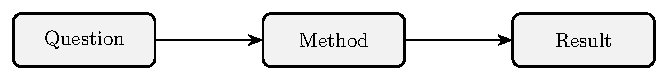
\includegraphics[width=\linewidth]{figures/example-diagram.pdf}
      \par\smallskip
      {\tiny 图注：替换为实际图形。}
  \end{columns}
\end{frame}

\begin{frame}{三栏等宽}
  \begin{columns}[T]
    \column{0.33\textwidth}
      \centering
      \textbf{阶段一}\\[6pt]
      描述第一阶段的核心特征或数据。
    \column{0.33\textwidth}
      \centering
      \textbf{阶段二}\\[6pt]
      描述第二阶段的核心特征或数据。
    \column{0.34\textwidth}
      \centering
      \textbf{阶段三}\\[6pt]
      描述第三阶段的核心特征或数据。
  \end{columns}
\end{frame}

% ------------------------------------------------------------------
\subsection{块与定理 / Blocks \& Theorems}
% ------------------------------------------------------------------

\begin{frame}{三种标准块}
  \begin{block}{标准块 (block)}
    用于关键事实、定义、或中性信息。
  \end{block}
  \begin{alertblock}{警示块 (alertblock)}
    用于警告、重要假设、或关键局限性。
  \end{alertblock}
  \begin{exampleblock}{示例块 (exampleblock)}
    用于数值例子、实证事实、或直觉说明。
  \end{exampleblock}
\end{frame}

\begin{frame}{定理与推论}
  \begin{theorem}[包络定理]
    设 $V(\theta) = \max_x f(x, \theta)$，则
    $\dfrac{dV}{d\theta} = \dfrac{\partial f}{\partial \theta}\big|_{x=x^*(\theta)}$。
  \end{theorem}
  \begin{corollary}
    在可微条件下，值函数关于参数的单调性由 $\partial f/\partial\theta$ 的符号决定。
  \end{corollary}
\end{frame}

\begin{frame}{定义与引理}
  \begin{definition}[纳什均衡]
    策略组合 $\sigma^*$ 是纳什均衡，当且仅当对任意参与人 $i$，
    在其他人策略不变的情况下，$i$ 无法通过单边偏离获益。
  \end{definition}
  \begin{lemma}
    任何有限博弈在混合策略意义下至少存在一个纳什均衡。
  \end{lemma}
\end{frame}

\begin{frame}{证明框架}
  \begin{proof}
    设 $x^* \notin \arg\max f(x)$，则存在 $x'$ 使得 $f(x') > f(x^*)$，
    与 $x^*$ 的最优性矛盾。故 $x^*$ 确为最大值点。
  \end{proof}
  \medskip
  \begin{exampleblock}{规范说明}
    Beamer 自动在 proof 结尾添加 $\square$，无需手动输入。
  \end{exampleblock}
\end{frame}

% ------------------------------------------------------------------
\subsection{数学公式 / Math}
% ------------------------------------------------------------------

\begin{frame}{行内与独行公式}
  行内公式：$\hat{\beta} = (X^\top X)^{-1} X^\top y$，
  或 $\text{plim}\,\hat{\beta} = \beta + (X^\top X/n)^{-1}(X^\top \varepsilon/n)$。

  \[
    \sigma^2 = \frac{1}{n}\sum_{i=1}^{n}(x_i - \bar{x})^2, \qquad
    \bar{x} = \frac{1}{n}\sum_{i=1}^{n} x_i.
  \]
\end{frame}

\begin{frame}{Align 带编号}
  \begin{align}
    \ell(\beta) &= \sum_{i=1}^{n}
      \bigl[y_i \log p_i + (1-y_i)\log(1-p_i)\bigr], \label{eq:loglik} \\
    \frac{\partial \ell}{\partial \beta} &= X^\top(y - p) = 0. \label{eq:foc}
  \end{align}
  式 \eqref{eq:loglik} 为对数似然；式 \eqref{eq:foc} 为一阶条件。
\end{frame}

\begin{frame}{矩阵}
  \[
    A = \begin{pmatrix} a_{11} & a_{12} \\ a_{21} & a_{22} \end{pmatrix}, \qquad
    B = \begin{bmatrix} 1 & 0 & 0 \\ 0 & 1 & 0 \\ 0 & 0 & 1 \end{bmatrix}, \qquad
    \det(A) = a_{11}a_{22} - a_{12}a_{21}.
  \]
\end{frame}

\begin{frame}{分段函数与 Cases}
  \[
    f(x) = \begin{cases}
      \alpha + \beta x   & \text{若 } x \geq \bar{x}, \\[4pt]
      \gamma + \delta x  & \text{若 } x < \bar{x}.
    \end{cases}
  \]
  \medskip
  注：用 \texttt{\\[4pt]} 在 cases 各行之间增加垂直间距。
\end{frame}

\begin{frame}{优化问题}
  \[
    \max_{\{c_t,\,k_{t+1}\}_{t=0}^{\infty}}
    \sum_{t=0}^{\infty} \beta^t u(c_t)
  \]
  \[
    \text{s.t.} \quad c_t + k_{t+1} = A k_t^\alpha, \quad
    c_t \geq 0, \quad k_0 \text{ 给定}.
  \]
  \begin{itemize}
    \item $\beta \in (0,1)$：折现因子；\quad $\alpha \in (0,1)$：资本份额。
    \item 贝尔曼方程：$V(k) = \max_{k'} \bigl\{u(Ak^\alpha - k') + \beta V(k')\bigr\}$。
  \end{itemize}
\end{frame}

% ------------------------------------------------------------------
\subsection{叠加动画 / Overlays \& Animations}
% ------------------------------------------------------------------

\begin{frame}{逐步显示：\texttt{\textbackslash pause}}
  \begin{itemize}
    \item 第一条：出现在第 1 页。
    \pause
    \item 第二条：出现在第 2 页。
    \pause
    \item 第三条：出现在第 3 页。
  \end{itemize}
  \pause
  \begin{exampleblock}{小结（第 4 页）}
    结合具体内容决定在何处插入 \texttt{\textbackslash pause}。
  \end{exampleblock}
\end{frame}

\begin{frame}{条件替换：\texttt{\textbackslash only}}
  \only<1>{
    \begin{block}{步骤 1 — 建模}
      定义参与人、策略空间和支付函数。
    \end{block}
  }
  \only<2>{
    \begin{block}{步骤 2 — 求解}
      对每位参与人求最优反应函数，联立求解。
    \end{block}
  }
  \only<3>{
    \begin{block}{步骤 3 — 解读}
      分析均衡的经济含义与福利性质。
    \end{block}
  }
  \vspace{0.5cm}
  \centering\footnotesize
  [\only<1>{第 1/3 页}\only<2>{第 2/3 页}\only<3>{第 3/3 页}]
\end{frame}

\begin{frame}{关键词逐步高亮：\texttt{\textbackslash alert<>}}
  估计策略分三步：
  \begin{itemize}
    \item<1-> \alert<1>{识别}：利用准随机变异剥离内生性。
    \item<2-> \alert<2>{估计}：对简约式做 OLS，获得降维方程。
    \item<3-> \alert<3>{推断}：使用聚类稳健标准误进行显著性检验。
  \end{itemize}
\end{frame}

\begin{frame}{未来条目置灰：\texttt{transparent}}
  {%  使用大括号将效果限制在本帧
    \setbeamercovered{transparent}
    \begin{itemize}
      \item<1-> 条目一（第 1 页完全可见，后续置灰）
      \item<2-> 条目二（第 2 页完全可见）
      \item<3-> 条目三（第 3 页完全可见）
    \end{itemize}
  }
\end{frame}

% ------------------------------------------------------------------
\subsection{图形与 TikZ / Figures \& TikZ}
% ------------------------------------------------------------------

\begin{frame}{并排双图（minipage）}
  \begin{columns}[c]
    \column{0.48\textwidth}
      \begin{figure}
        \centering
        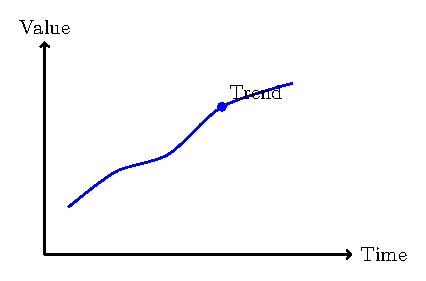
\includegraphics[width=\linewidth,height=0.48\textheight,
                         keepaspectratio]{figures/example-chart.pdf}
        \caption{面板 A：处理组}
      \end{figure}
    \column{0.48\textwidth}
      \begin{figure}
        \centering
        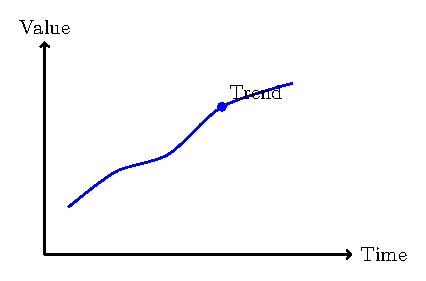
\includegraphics[width=\linewidth,height=0.48\textheight,
                         keepaspectratio]{figures/example-chart.pdf}
        \caption{面板 B：对照组}
      \end{figure}
  \end{columns}
\end{frame}

\begin{frame}{TikZ — 因果有向图 (DAG)}
  \centering
  \begin{tikzpicture}[
      node distance=1.8cm and 2.6cm,
      box/.style={draw, rounded corners=4pt,
                  minimum width=1.9cm, minimum height=0.65cm,
                  font=\small, fill=white},
      >=Stealth, thick
    ]
    \node[box] (Z) {工具变量 $Z$};
    \node[box, right=of Z] (X) {处理变量 $X$};
    \node[box, right=of X] (Y) {结果变量 $Y$};
    \node[box, dashed, above right=0.55cm and 0.9cm of X]
          (U) {不可观测 $U$};
    \draw[->] (Z) -- (X);
    \draw[->] (X) -- (Y);
    \draw[->, dashed, gray] (U) -- (X);
    \draw[->, dashed, gray] (U) -- (Y);
    \draw[->, red!70!black, bend right=18]
          node[below, font=\scriptsize, midway]{排除限制} (Z.south) to (Y.south);
    % 注：上面的 bend right 箭头演示"违反排除限制"的情形，
    %     实际使用时可删去。
  \end{tikzpicture}
  \par\smallskip
  {\footnotesize 虚线 = 不可观测路径；红色弯箭头 = 违反排除限制（示意）。}
\end{frame}

\begin{frame}{TikZ — 流程图}
  \centering
  \begin{tikzpicture}[
      node distance=0.75cm,
      box/.style={draw, rounded corners=3pt,
                  minimum width=3.4cm, minimum height=0.58cm,
                  align=center, font=\small, fill=blue!5},
      dec/.style={draw, diamond, aspect=2.6,
                  minimum width=2.8cm, font=\small, fill=orange!10},
      >=Stealth, thick
    ]
    \node[box]  (data)  {原始数据};
    \node[box, below=of data]  (clean) {清洗与预处理};
    \node[dec, below=of clean] (valid) {通过质检？};
    \node[box, below=of valid] (est)   {模型估计};
    \node[box, below=of est]   (rep)   {报告结果};

    \draw[->] (data)  -- (clean);
    \draw[->] (clean) -- (valid);
    \draw[->] (valid) -- node[right, font=\scriptsize]{是} (est);
    \draw[->] (valid.west) -- ++(-1.3,0)
              |- node[left, font=\scriptsize, pos=0.22]{否} (clean.west);
    \draw[->] (est)   -- (rep);
  \end{tikzpicture}
\end{frame}
\begin{frame}{TikZ — 水平时间轴}
  \centering
  \begin{tikzpicture}[>=Stealth, thick, font=\small]
    
    % 1. 调整背景框的深度（下移至 -0.85）
    \fill[blue!15, rounded corners=2pt] (2.2,-0.55) rectangle (6.8, 0.05);
    % 2. 将“样本期间”文字下移（Y坐标从 -0.35 改为 -0.65），避开“2008”
    \node[font=\scriptsize, text=blue!60!black] at (4.5,-0.65) {样本期间};

    % 3. 绘制主时间轴和年份刻度
    \draw[->] (-0.3,0) -- (9.2,0) node[right] {年份};
    \foreach \x/\yr in {0.5/1990, 2.5/2000, 4.5/2008, 6.5/2015, 8.5/2023}{
      \draw (\x, 0.12) -- (\x,-0.12) node[below] {\yr};
    }
    
    % 4. 事件标注（上方）
    \node[above, align=center, font=\scriptsize] at (0.5, 0.22) {改革 A};
    \node[above, align=center, font=\scriptsize] at (2.5, 0.22) {改革 B};
    \node[above, align=center, font=\scriptsize, text=red!70!black]
          at (4.5, 0.22) {金融危机};
    \node[above, align=center, font=\scriptsize] at (6.5, 0.22) {政策 C};
    \node[above, align=center, font=\scriptsize] at (8.5, 0.22) {今日};
    
    % 5. 当前位置标记
    \draw[red!70!black, thick] (8.5,0.35) -- (8.5,-0.12);
    
  \end{tikzpicture}
\end{frame}
% ------------------------------------------------------------------
\subsection{表格样例 / Tables}
% ------------------------------------------------------------------

\begin{frame}{描述性统计}
  \input{tables/summary-stats}
\end{frame}

\begin{frame}{多列回归比较}
  \input{tables/reg-comparison}
\end{frame}

\begin{frame}[shrink=20]{双面板（Panel A / B）异质性}
  \input{tables/twopart-table}
\end{frame}

\begin{frame}{行高亮表格（colortbl）}
  % 需要在 main.tex 中加载 \usepackage{colortbl}
  \begin{table}
    \centering
    \caption{带高亮行的表格示例}
    \begin{tabular}{lcc}
      \toprule
      变量 & 处理组 & 对照组 \\
      \midrule
      \rowcolor{yellow!30}
      GDP 增速 (\%) & 6.8 & 3.2 \\
      失业率 (\%)   & 4.1 & 7.6 \\
      \rowcolor{yellow!30}
      通货膨胀 (\%) & 2.3 & 4.8 \\
      贸易开放度    & 0.72 & 0.51 \\
      \bottomrule
    \end{tabular}
  \end{table}
  {\footnotesize \textit{注}：黄色行为核心关注变量。}
\end{frame}

% ------------------------------------------------------------------
\subsection{代码与逐字排版 / Code \& Verbatim}
% ------------------------------------------------------------------

\begin{frame}[fragile]{Python 代码（listings）}
  % 需要在 main.tex 中加载 \usepackage{listings} 并配置 \lstset
  \begin{lstlisting}[language=Python, caption={OLS 估计量（NumPy 实现）}]
import numpy as np

def ols(X, y):
    """返回 OLS 系数向量 beta_hat."""
    return np.linalg.solve(X.T @ X, X.T @ y)

# 生成模拟数据
rng  = np.random.default_rng(42)
X    = np.column_stack([np.ones(200), rng.standard_normal((200, 2))])
beta = np.array([1.0, 2.0, -0.5])
y    = X @ beta + rng.standard_normal(200)

print(ols(X, y))   # 应接近 [1, 2, -0.5]
  \end{lstlisting}
\end{frame}

\begin{frame}[fragile]{LaTeX 代码排版（lstlisting）}
  % ⚠ Beamer 限制：[fragile] 帧的内容（含 \input 子文件）里
  %   不能出现字面的 \end{frame}，否则 Beamer 预扫描会误判帧结束。
  %   解决方法：只展示帧内部代码，外层 \begin/\end{frame} 用文字说明。
  \begin{lstlisting}[language=TeX, caption={帧内叠加动画（内部代码）}]
% 以下内容放在 frame 环境内部（外层为 \begin{frame}...\end{...} 结构）：
\begin{itemize}
  \item<1-> \alert<1>{Step 1}: 建立模型
  \item<2-> \alert<2>{Step 2}: 求解均衡
  \item<3-> \alert<3>{Step 3}: 实证检验
\end{itemize}
\setbeamercovered{transparent}  % 未到场条目置灰
  \end{lstlisting}
  {\footnotesize\textit{注}：若需在代码块中展示完整帧结构（含 \texttt{\textbackslash end\{frame\}}），
  可将代码存入独立 \texttt{.tex} 文件后用 \texttt{\textbackslash lstinputlisting} 引入。}
\end{frame}

% ------------------------------------------------------------------
\subsection{特殊幻灯片与导航 / Special Slides \& Navigation}
% ------------------------------------------------------------------

\begin{frame}{章节过渡页}
  \vspace*{\fill}
  \begin{center}
    {\Large \textbf{第~\Roman{section}~部分}}\\[0.7em]
    {\large \insertsectionhead}\\[1.2em]
    {\normalsize 一句话预告本节核心内容。}
  \end{center}
  \vspace*{\fill}
\end{frame}

\begin{frame}{进度路线图（手动高亮当前节）}
  \begin{enumerate}
    \item[\checkmark] 引言
    \item[\checkmark] 背景与文献
    \item[\textbf{3.}] \textbf{模型} \quad \textcolor{blue}{$\leftarrow$ 当前}
    \item[4.] \textcolor{gray}{实证分析}
    \item[5.] \textcolor{gray}{结论}
  \end{enumerate}
\end{frame}

\begin{frame}{两箱对比（alertblock vs exampleblock）}
  \begin{columns}[T]
    \column{0.48\textwidth}
      \begin{alertblock}{无干预（基准）}
        \begin{itemize}
          \item 产出增速：低
          \item 失业率：高
          \item 社会福利：$W_0$
        \end{itemize}
      \end{alertblock}
    \column{0.48\textwidth}
      \begin{exampleblock}{有干预（反事实）}
        \begin{itemize}
          \item 产出增速：高
          \item 失业率：低
          \item 社会福利：$W_1 > W_0$
        \end{itemize}
      \end{exampleblock}
  \end{columns}
\end{frame}

\begin{frame}{引言页 / Pull Quote}
  \vspace*{\fill}
  \begin{center}
    \Large\itshape
    ``好的模型不求包罗万象，\\
    只求能对关键机制给出清晰预测。''
    \vspace{0.9em}

    \normalsize\upshape
    --- 示例引用，\textit{来源书目}，年份
  \end{center}
  \vspace*{\fill}
\end{frame}

% 超链接导航示例
% 用法：目标帧内加 \label{frm:target}，此处用 \hyperlink{frm:target}{按钮}
\begin{frame}{附录跳转按钮}
  正文幻灯片可加入指向附录的按钮，听众提问时快速跳转：

  \medskip
  \hyperlink{frm:robustness}{\beamergotobutton{稳健性检验}}
  \hspace{1em}
  \hyperlink{frm:derivation}{\beamergotobutton{完整推导}}
  \hspace{1em}
  \hyperlink{frm:data}{\beamergotobutton{数据说明}}

  \bigskip
  附录帧返回正文：

  \medskip
  \hyperlink{frm:main-results}{\beamerreturnbutton{返回主结果}}
  \hspace{1em}
  \hyperlink{frm:empirics}{\beamerbutton{跳至实证节}}

  \bigskip
  {\footnotesize \textit{用法}：在目标帧内加
    \texttt{\textbackslash label\{frm:robustness\}} 等标签即可激活以上按钮。}
\end{frame}

%  即可将本库编译进文档。
% ============================================================

\section{Slide Gallery}

% ------------------------------------------------------------------
\subsection{文字与列表 / Text \& Lists}
% ------------------------------------------------------------------

\begin{frame}{Itemize — 三级嵌套}
  \begin{itemize}
    \item 一级条目（默认样式）
      \begin{itemize}
        \item 二级条目（缩进更深）
          \begin{itemize}
            \item 三级条目（通常避免超过三级）
          \end{itemize}
      \end{itemize}
    \item 另一条一级条目
    \item 再一条一级条目
  \end{itemize}
\end{frame}

\begin{frame}{Enumerate — 有序列表}
  \begin{enumerate}
    \item 第一步：提出问题
    \item 第二步：建立模型
      \begin{enumerate}
        \item 子步骤 A
        \item 子步骤 B
      \end{enumerate}
    \item 第三步：实证检验
    \item 第四步：政策含义
  \end{enumerate}
\end{frame}

\begin{frame}{Description — 术语表}
  \begin{description}
    \item[识别 (Identification)] 将因果效应与相关性分离的策略。
    \item[工具变量 (IV)] 影响处理变量但不直接影响结果的变量。
    \item[排除限制 (Exclusion)] 工具变量仅通过处理变量影响结果。
    \item[外生性 (Exogeneity)] 工具变量与误差项不相关的假设。
  \end{description}
\end{frame}

\begin{frame}{强调与颜色}
  \begin{itemize}
    \item 使用 \alert{alert} 将关键词标红（beamer 默认强调色）。
    \item 使用 \textbf{粗体}表示重要概念。
    \item 使用 \textit{斜体}表示书名、外文词汇。
    \item 使用 \textcolor{blue}{自定义颜色}：\texttt{\textbackslash textcolor\{blue\}\{...\}}。
    \item 使用 \colorbox{yellow!40}{背景高亮}：\texttt{\textbackslash colorbox\{yellow!40\}\{...\}}。
    \item \structure{结构色}（beamer \texttt{\textbackslash structure}）跟随主题变化。
  \end{itemize}
\end{frame}

% ------------------------------------------------------------------
\subsection{分栏布局 / Column Layouts}
% ------------------------------------------------------------------

\begin{frame}{两栏均等 50/50}
  \begin{columns}[T]
    \column{0.5\textwidth}
      \textbf{左栏}
      \begin{itemize}
        \item 论点一
        \item 论点二
        \item 论点三
      \end{itemize}
    \column{0.5\textwidth}
      \textbf{右栏}
      \begin{itemize}
        \item 反驳一
        \item 反驳二
        \item 反驳三
      \end{itemize}
  \end{columns}
\end{frame}

\begin{frame}{两栏不等 60/40（文字 + 图）}
  \begin{columns}[T]
    \column{0.60\textwidth}
      \begin{itemize}
        \item 宽栏放主要论述，窄栏放配图或摘要。
        \item 保持每条 bullet 简短，避免折行过多。
        \item 此布局适合"文字驱动"幻灯片。
      \end{itemize}
    \column{0.40\textwidth}
      \centering
      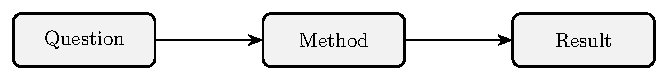
\includegraphics[width=\linewidth]{figures/example-diagram.pdf}
      \par\smallskip
      {\tiny 图注：替换为实际图形。}
  \end{columns}
\end{frame}

\begin{frame}{三栏等宽}
  \begin{columns}[T]
    \column{0.33\textwidth}
      \centering
      \textbf{阶段一}\\[6pt]
      描述第一阶段的核心特征或数据。
    \column{0.33\textwidth}
      \centering
      \textbf{阶段二}\\[6pt]
      描述第二阶段的核心特征或数据。
    \column{0.34\textwidth}
      \centering
      \textbf{阶段三}\\[6pt]
      描述第三阶段的核心特征或数据。
  \end{columns}
\end{frame}

% ------------------------------------------------------------------
\subsection{块与定理 / Blocks \& Theorems}
% ------------------------------------------------------------------

\begin{frame}{三种标准块}
  \begin{block}{标准块 (block)}
    用于关键事实、定义、或中性信息。
  \end{block}
  \begin{alertblock}{警示块 (alertblock)}
    用于警告、重要假设、或关键局限性。
  \end{alertblock}
  \begin{exampleblock}{示例块 (exampleblock)}
    用于数值例子、实证事实、或直觉说明。
  \end{exampleblock}
\end{frame}

\begin{frame}{定理与推论}
  \begin{theorem}[包络定理]
    设 $V(\theta) = \max_x f(x, \theta)$，则
    $\dfrac{dV}{d\theta} = \dfrac{\partial f}{\partial \theta}\big|_{x=x^*(\theta)}$。
  \end{theorem}
  \begin{corollary}
    在可微条件下，值函数关于参数的单调性由 $\partial f/\partial\theta$ 的符号决定。
  \end{corollary}
\end{frame}

\begin{frame}{定义与引理}
  \begin{definition}[纳什均衡]
    策略组合 $\sigma^*$ 是纳什均衡，当且仅当对任意参与人 $i$，
    在其他人策略不变的情况下，$i$ 无法通过单边偏离获益。
  \end{definition}
  \begin{lemma}
    任何有限博弈在混合策略意义下至少存在一个纳什均衡。
  \end{lemma}
\end{frame}

\begin{frame}{证明框架}
  \begin{proof}
    设 $x^* \notin \arg\max f(x)$，则存在 $x'$ 使得 $f(x') > f(x^*)$，
    与 $x^*$ 的最优性矛盾。故 $x^*$ 确为最大值点。
  \end{proof}
  \medskip
  \begin{exampleblock}{规范说明}
    Beamer 自动在 proof 结尾添加 $\square$，无需手动输入。
  \end{exampleblock}
\end{frame}

% ------------------------------------------------------------------
\subsection{数学公式 / Math}
% ------------------------------------------------------------------

\begin{frame}{行内与独行公式}
  行内公式：$\hat{\beta} = (X^\top X)^{-1} X^\top y$，
  或 $\text{plim}\,\hat{\beta} = \beta + (X^\top X/n)^{-1}(X^\top \varepsilon/n)$。

  \[
    \sigma^2 = \frac{1}{n}\sum_{i=1}^{n}(x_i - \bar{x})^2, \qquad
    \bar{x} = \frac{1}{n}\sum_{i=1}^{n} x_i.
  \]
\end{frame}

\begin{frame}{Align 带编号}
  \begin{align}
    \ell(\beta) &= \sum_{i=1}^{n}
      \bigl[y_i \log p_i + (1-y_i)\log(1-p_i)\bigr], \label{eq:loglik} \\
    \frac{\partial \ell}{\partial \beta} &= X^\top(y - p) = 0. \label{eq:foc}
  \end{align}
  式 \eqref{eq:loglik} 为对数似然；式 \eqref{eq:foc} 为一阶条件。
\end{frame}

\begin{frame}{矩阵}
  \[
    A = \begin{pmatrix} a_{11} & a_{12} \\ a_{21} & a_{22} \end{pmatrix}, \qquad
    B = \begin{bmatrix} 1 & 0 & 0 \\ 0 & 1 & 0 \\ 0 & 0 & 1 \end{bmatrix}, \qquad
    \det(A) = a_{11}a_{22} - a_{12}a_{21}.
  \]
\end{frame}

\begin{frame}{分段函数与 Cases}
  \[
    f(x) = \begin{cases}
      \alpha + \beta x   & \text{若 } x \geq \bar{x}, \\[4pt]
      \gamma + \delta x  & \text{若 } x < \bar{x}.
    \end{cases}
  \]
  \medskip
  注：用 \texttt{\\[4pt]} 在 cases 各行之间增加垂直间距。
\end{frame}

\begin{frame}{优化问题}
  \[
    \max_{\{c_t,\,k_{t+1}\}_{t=0}^{\infty}}
    \sum_{t=0}^{\infty} \beta^t u(c_t)
  \]
  \[
    \text{s.t.} \quad c_t + k_{t+1} = A k_t^\alpha, \quad
    c_t \geq 0, \quad k_0 \text{ 给定}.
  \]
  \begin{itemize}
    \item $\beta \in (0,1)$：折现因子；\quad $\alpha \in (0,1)$：资本份额。
    \item 贝尔曼方程：$V(k) = \max_{k'} \bigl\{u(Ak^\alpha - k') + \beta V(k')\bigr\}$。
  \end{itemize}
\end{frame}

% ------------------------------------------------------------------
\subsection{叠加动画 / Overlays \& Animations}
% ------------------------------------------------------------------

\begin{frame}{逐步显示：\texttt{\textbackslash pause}}
  \begin{itemize}
    \item 第一条：出现在第 1 页。
    \pause
    \item 第二条：出现在第 2 页。
    \pause
    \item 第三条：出现在第 3 页。
  \end{itemize}
  \pause
  \begin{exampleblock}{小结（第 4 页）}
    结合具体内容决定在何处插入 \texttt{\textbackslash pause}。
  \end{exampleblock}
\end{frame}

\begin{frame}{条件替换：\texttt{\textbackslash only}}
  \only<1>{
    \begin{block}{步骤 1 — 建模}
      定义参与人、策略空间和支付函数。
    \end{block}
  }
  \only<2>{
    \begin{block}{步骤 2 — 求解}
      对每位参与人求最优反应函数，联立求解。
    \end{block}
  }
  \only<3>{
    \begin{block}{步骤 3 — 解读}
      分析均衡的经济含义与福利性质。
    \end{block}
  }
  \vspace{0.5cm}
  \centering\footnotesize
  [\only<1>{第 1/3 页}\only<2>{第 2/3 页}\only<3>{第 3/3 页}]
\end{frame}

\begin{frame}{关键词逐步高亮：\texttt{\textbackslash alert<>}}
  估计策略分三步：
  \begin{itemize}
    \item<1-> \alert<1>{识别}：利用准随机变异剥离内生性。
    \item<2-> \alert<2>{估计}：对简约式做 OLS，获得降维方程。
    \item<3-> \alert<3>{推断}：使用聚类稳健标准误进行显著性检验。
  \end{itemize}
\end{frame}

\begin{frame}{未来条目置灰：\texttt{transparent}}
  {%  使用大括号将效果限制在本帧
    \setbeamercovered{transparent}
    \begin{itemize}
      \item<1-> 条目一（第 1 页完全可见，后续置灰）
      \item<2-> 条目二（第 2 页完全可见）
      \item<3-> 条目三（第 3 页完全可见）
    \end{itemize}
  }
\end{frame}

% ------------------------------------------------------------------
\subsection{图形与 TikZ / Figures \& TikZ}
% ------------------------------------------------------------------

\begin{frame}{并排双图（minipage）}
  \begin{columns}[c]
    \column{0.48\textwidth}
      \begin{figure}
        \centering
        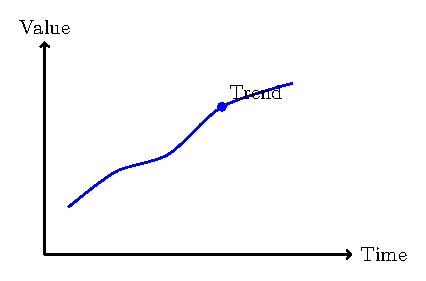
\includegraphics[width=\linewidth,height=0.48\textheight,
                         keepaspectratio]{figures/example-chart.pdf}
        \caption{面板 A：处理组}
      \end{figure}
    \column{0.48\textwidth}
      \begin{figure}
        \centering
        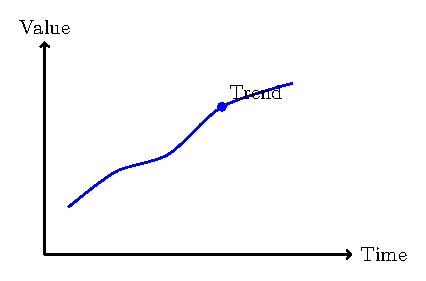
\includegraphics[width=\linewidth,height=0.48\textheight,
                         keepaspectratio]{figures/example-chart.pdf}
        \caption{面板 B：对照组}
      \end{figure}
  \end{columns}
\end{frame}

\begin{frame}{TikZ — 因果有向图 (DAG)}
  \centering
  \begin{tikzpicture}[
      node distance=1.8cm and 2.6cm,
      box/.style={draw, rounded corners=4pt,
                  minimum width=1.9cm, minimum height=0.65cm,
                  font=\small, fill=white},
      >=Stealth, thick
    ]
    \node[box] (Z) {工具变量 $Z$};
    \node[box, right=of Z] (X) {处理变量 $X$};
    \node[box, right=of X] (Y) {结果变量 $Y$};
    \node[box, dashed, above right=0.55cm and 0.9cm of X]
          (U) {不可观测 $U$};
    \draw[->] (Z) -- (X);
    \draw[->] (X) -- (Y);
    \draw[->, dashed, gray] (U) -- (X);
    \draw[->, dashed, gray] (U) -- (Y);
    \draw[->, red!70!black, bend right=18]
          node[below, font=\scriptsize, midway]{排除限制} (Z.south) to (Y.south);
    % 注：上面的 bend right 箭头演示"违反排除限制"的情形，
    %     实际使用时可删去。
  \end{tikzpicture}
  \par\smallskip
  {\footnotesize 虚线 = 不可观测路径；红色弯箭头 = 违反排除限制（示意）。}
\end{frame}

\begin{frame}{TikZ — 流程图}
  \centering
  \begin{tikzpicture}[
      node distance=0.75cm,
      box/.style={draw, rounded corners=3pt,
                  minimum width=3.4cm, minimum height=0.58cm,
                  align=center, font=\small, fill=blue!5},
      dec/.style={draw, diamond, aspect=2.6,
                  minimum width=2.8cm, font=\small, fill=orange!10},
      >=Stealth, thick
    ]
    \node[box]  (data)  {原始数据};
    \node[box, below=of data]  (clean) {清洗与预处理};
    \node[dec, below=of clean] (valid) {通过质检？};
    \node[box, below=of valid] (est)   {模型估计};
    \node[box, below=of est]   (rep)   {报告结果};

    \draw[->] (data)  -- (clean);
    \draw[->] (clean) -- (valid);
    \draw[->] (valid) -- node[right, font=\scriptsize]{是} (est);
    \draw[->] (valid.west) -- ++(-1.3,0)
              |- node[left, font=\scriptsize, pos=0.22]{否} (clean.west);
    \draw[->] (est)   -- (rep);
  \end{tikzpicture}
\end{frame}
\begin{frame}{TikZ — 水平时间轴}
  \centering
  \begin{tikzpicture}[>=Stealth, thick, font=\small]
    
    % 1. 调整背景框的深度（下移至 -0.85）
    \fill[blue!15, rounded corners=2pt] (2.2,-0.55) rectangle (6.8, 0.05);
    % 2. 将“样本期间”文字下移（Y坐标从 -0.35 改为 -0.65），避开“2008”
    \node[font=\scriptsize, text=blue!60!black] at (4.5,-0.65) {样本期间};

    % 3. 绘制主时间轴和年份刻度
    \draw[->] (-0.3,0) -- (9.2,0) node[right] {年份};
    \foreach \x/\yr in {0.5/1990, 2.5/2000, 4.5/2008, 6.5/2015, 8.5/2023}{
      \draw (\x, 0.12) -- (\x,-0.12) node[below] {\yr};
    }
    
    % 4. 事件标注（上方）
    \node[above, align=center, font=\scriptsize] at (0.5, 0.22) {改革 A};
    \node[above, align=center, font=\scriptsize] at (2.5, 0.22) {改革 B};
    \node[above, align=center, font=\scriptsize, text=red!70!black]
          at (4.5, 0.22) {金融危机};
    \node[above, align=center, font=\scriptsize] at (6.5, 0.22) {政策 C};
    \node[above, align=center, font=\scriptsize] at (8.5, 0.22) {今日};
    
    % 5. 当前位置标记
    \draw[red!70!black, thick] (8.5,0.35) -- (8.5,-0.12);
    
  \end{tikzpicture}
\end{frame}
% ------------------------------------------------------------------
\subsection{表格样例 / Tables}
% ------------------------------------------------------------------

\begin{frame}{描述性统计}
  \begin{table}
  \centering
  \caption{描述性统计（Summary Statistics）}
  {\small
  \begin{tabular}{lrrrr}
    \toprule
    变量 & 均值 & 标准差 & 最小值 & 最大值 \\
    \midrule
    人均 GDP（美元）       & 12{,}450 & 3{,}821 & 5{,}200  & 24{,}100 \\
    失业率（\%）           &     6.2  &    2.1  &     1.8  &     14.3 \\
    通货膨胀率（\%）       &     3.4  &    1.9  &  $-$0.5  &     11.2 \\
    贸易开放度             &    0.68  &   0.22  &    0.12  &      1.45 \\
    城镇化率（\%）         &    56.3  &   14.7  &    22.0  &     89.4 \\
    人力资本指数           &     2.8  &    0.6  &     1.5  &      4.1 \\
    \midrule
    样本量 $N$             & \multicolumn{4}{c}{1{,}200} \\
    \bottomrule
  \end{tabular}}
  \par\smallskip
  \raggedright
  {\footnotesize \textit{注}：年度面板数据，2000--2020 年。
  样本限于人口超过 100 万的国家。}
\end{table}

\end{frame}

\begin{frame}{多列回归比较}
  \begin{table}
  \centering
  \caption{回归结果：四种设定（Regression Results）}
  {\scriptsize
  \begin{tabular}{lcccc}
    \toprule
    & (1) OLS & (2) OLS & (3) IV & (4) IV \\
    & 基准    & +控制变量 & 基准  & +控制变量 \\
    \midrule
    处理变量          & 0.125*** & 0.098**  & 0.187*** & 0.142** \\
                      & (0.031)  & (0.040)  & (0.055)  & (0.063) \\[4pt]
    对数收入          &          & 0.234*** &          & 0.211*** \\
                      &          & (0.022)  &          & (0.025) \\[4pt]
    教育年限          &          & 0.044*   &          & 0.039*  \\
                      &          & (0.024)  &          & (0.022) \\
    \midrule
    控制变量          & 否  & 是  & 否  & 是  \\
    固定效应          & 否  & 是  & 否  & 是  \\
    $N$               & 1{,}200 & 1{,}200 & 1{,}200 & 1{,}200 \\
    $R^2$             & 0.18 & 0.34 & --- & --- \\
    F 统计（弱工具）  &      &      & 18.7 & 21.3 \\
    \bottomrule
    \multicolumn{5}{l}{%
      \scriptsize
      *** $p<0.01$，** $p<0.05$，* $p<0.1$。括号内为聚类稳健标准误。}
  \end{tabular}}
\end{table}

\end{frame}

\begin{frame}[shrink=20]{双面板（Panel A / B）异质性}
  \begin{table}
  \centering
  \caption{异质性分析：双面板（Two-Panel Heterogeneity）}
  {\footnotesize
  \begin{tabular}{lcc}
    \toprule
    & (1) 低收入组 & (2) 高收入组 \\
    \midrule
    \multicolumn{3}{l}{\textit{面板 A：城市样本}} \\
    \midrule
    处理效应   & 0.142**  & 0.098*   \\
               & (0.058)  & (0.052)  \\
    控制变量   & 是       & 是       \\
    $N$        & 600      & 600      \\
    \midrule
    \multicolumn{3}{l}{\textit{面板 B：农村样本}} \\
    \midrule
    处理效应   & 0.072    & 0.031    \\
               & (0.074)  & (0.069)  \\
    控制变量   & 是       & 是       \\
    $N$        & 400      & 400      \\
    \midrule
    \multicolumn{3}{l}{\textit{面板差异（A $-$ B）}} \\
    \midrule
    差值       & 0.070    & 0.067    \\
    $p$ 值     & 0.043    & 0.061    \\
    \bottomrule
    \multicolumn{3}{l}{%
      \footnotesize ** $p<0.05$，* $p<0.1$。括号内为聚类稳健标准误。}
  \end{tabular}}
\end{table}

\end{frame}

\begin{frame}{行高亮表格（colortbl）}
  % 需要在 main.tex 中加载 \usepackage{colortbl}
  \begin{table}
    \centering
    \caption{带高亮行的表格示例}
    \begin{tabular}{lcc}
      \toprule
      变量 & 处理组 & 对照组 \\
      \midrule
      \rowcolor{yellow!30}
      GDP 增速 (\%) & 6.8 & 3.2 \\
      失业率 (\%)   & 4.1 & 7.6 \\
      \rowcolor{yellow!30}
      通货膨胀 (\%) & 2.3 & 4.8 \\
      贸易开放度    & 0.72 & 0.51 \\
      \bottomrule
    \end{tabular}
  \end{table}
  {\footnotesize \textit{注}：黄色行为核心关注变量。}
\end{frame}

% ------------------------------------------------------------------
\subsection{代码与逐字排版 / Code \& Verbatim}
% ------------------------------------------------------------------

\begin{frame}[fragile]{Python 代码（listings）}
  % 需要在 main.tex 中加载 \usepackage{listings} 并配置 \lstset
  \begin{lstlisting}[language=Python, caption={OLS 估计量（NumPy 实现）}]
import numpy as np

def ols(X, y):
    """返回 OLS 系数向量 beta_hat."""
    return np.linalg.solve(X.T @ X, X.T @ y)

# 生成模拟数据
rng  = np.random.default_rng(42)
X    = np.column_stack([np.ones(200), rng.standard_normal((200, 2))])
beta = np.array([1.0, 2.0, -0.5])
y    = X @ beta + rng.standard_normal(200)

print(ols(X, y))   # 应接近 [1, 2, -0.5]
  \end{lstlisting}
\end{frame}

\begin{frame}[fragile]{LaTeX 代码排版（lstlisting）}
  % ⚠ Beamer 限制：[fragile] 帧的内容（含 \input 子文件）里
  %   不能出现字面的 \end{frame}，否则 Beamer 预扫描会误判帧结束。
  %   解决方法：只展示帧内部代码，外层 \begin/\end{frame} 用文字说明。
  \begin{lstlisting}[language=TeX, caption={帧内叠加动画（内部代码）}]
% 以下内容放在 frame 环境内部（外层为 \begin{frame}...\end{...} 结构）：
\begin{itemize}
  \item<1-> \alert<1>{Step 1}: 建立模型
  \item<2-> \alert<2>{Step 2}: 求解均衡
  \item<3-> \alert<3>{Step 3}: 实证检验
\end{itemize}
\setbeamercovered{transparent}  % 未到场条目置灰
  \end{lstlisting}
  {\footnotesize\textit{注}：若需在代码块中展示完整帧结构（含 \texttt{\textbackslash end\{frame\}}），
  可将代码存入独立 \texttt{.tex} 文件后用 \texttt{\textbackslash lstinputlisting} 引入。}
\end{frame}

% ------------------------------------------------------------------
\subsection{特殊幻灯片与导航 / Special Slides \& Navigation}
% ------------------------------------------------------------------

\begin{frame}{章节过渡页}
  \vspace*{\fill}
  \begin{center}
    {\Large \textbf{第~\Roman{section}~部分}}\\[0.7em]
    {\large \insertsectionhead}\\[1.2em]
    {\normalsize 一句话预告本节核心内容。}
  \end{center}
  \vspace*{\fill}
\end{frame}

\begin{frame}{进度路线图（手动高亮当前节）}
  \begin{enumerate}
    \item[\checkmark] 引言
    \item[\checkmark] 背景与文献
    \item[\textbf{3.}] \textbf{模型} \quad \textcolor{blue}{$\leftarrow$ 当前}
    \item[4.] \textcolor{gray}{实证分析}
    \item[5.] \textcolor{gray}{结论}
  \end{enumerate}
\end{frame}

\begin{frame}{两箱对比（alertblock vs exampleblock）}
  \begin{columns}[T]
    \column{0.48\textwidth}
      \begin{alertblock}{无干预（基准）}
        \begin{itemize}
          \item 产出增速：低
          \item 失业率：高
          \item 社会福利：$W_0$
        \end{itemize}
      \end{alertblock}
    \column{0.48\textwidth}
      \begin{exampleblock}{有干预（反事实）}
        \begin{itemize}
          \item 产出增速：高
          \item 失业率：低
          \item 社会福利：$W_1 > W_0$
        \end{itemize}
      \end{exampleblock}
  \end{columns}
\end{frame}

\begin{frame}{引言页 / Pull Quote}
  \vspace*{\fill}
  \begin{center}
    \Large\itshape
    ``好的模型不求包罗万象，\\
    只求能对关键机制给出清晰预测。''
    \vspace{0.9em}

    \normalsize\upshape
    --- 示例引用，\textit{来源书目}，年份
  \end{center}
  \vspace*{\fill}
\end{frame}

% 超链接导航示例
% 用法：目标帧内加 \label{frm:target}，此处用 \hyperlink{frm:target}{按钮}
\begin{frame}{附录跳转按钮}
  正文幻灯片可加入指向附录的按钮，听众提问时快速跳转：

  \medskip
  \hyperlink{frm:robustness}{\beamergotobutton{稳健性检验}}
  \hspace{1em}
  \hyperlink{frm:derivation}{\beamergotobutton{完整推导}}
  \hspace{1em}
  \hyperlink{frm:data}{\beamergotobutton{数据说明}}

  \bigskip
  附录帧返回正文：

  \medskip
  \hyperlink{frm:main-results}{\beamerreturnbutton{返回主结果}}
  \hspace{1em}
  \hyperlink{frm:empirics}{\beamerbutton{跳至实证节}}

  \bigskip
  {\footnotesize \textit{用法}：在目标帧内加
    \texttt{\textbackslash label\{frm:robustness\}} 等标签即可激活以上按钮。}
\end{frame}

%  即可将本库编译进文档。
% ============================================================

\section{Slide Gallery}

% ------------------------------------------------------------------
\subsection{文字与列表 / Text \& Lists}
% ------------------------------------------------------------------

\begin{frame}{Itemize — 三级嵌套}
  \begin{itemize}
    \item 一级条目（默认样式）
      \begin{itemize}
        \item 二级条目（缩进更深）
          \begin{itemize}
            \item 三级条目（通常避免超过三级）
          \end{itemize}
      \end{itemize}
    \item 另一条一级条目
    \item 再一条一级条目
  \end{itemize}
\end{frame}

\begin{frame}{Enumerate — 有序列表}
  \begin{enumerate}
    \item 第一步：提出问题
    \item 第二步：建立模型
      \begin{enumerate}
        \item 子步骤 A
        \item 子步骤 B
      \end{enumerate}
    \item 第三步：实证检验
    \item 第四步：政策含义
  \end{enumerate}
\end{frame}

\begin{frame}{Description — 术语表}
  \begin{description}
    \item[识别 (Identification)] 将因果效应与相关性分离的策略。
    \item[工具变量 (IV)] 影响处理变量但不直接影响结果的变量。
    \item[排除限制 (Exclusion)] 工具变量仅通过处理变量影响结果。
    \item[外生性 (Exogeneity)] 工具变量与误差项不相关的假设。
  \end{description}
\end{frame}

\begin{frame}{强调与颜色}
  \begin{itemize}
    \item 使用 \alert{alert} 将关键词标红（beamer 默认强调色）。
    \item 使用 \textbf{粗体}表示重要概念。
    \item 使用 \textit{斜体}表示书名、外文词汇。
    \item 使用 \textcolor{blue}{自定义颜色}：\texttt{\textbackslash textcolor\{blue\}\{...\}}。
    \item 使用 \colorbox{yellow!40}{背景高亮}：\texttt{\textbackslash colorbox\{yellow!40\}\{...\}}。
    \item \structure{结构色}（beamer \texttt{\textbackslash structure}）跟随主题变化。
  \end{itemize}
\end{frame}

% ------------------------------------------------------------------
\subsection{分栏布局 / Column Layouts}
% ------------------------------------------------------------------

\begin{frame}{两栏均等 50/50}
  \begin{columns}[T]
    \column{0.5\textwidth}
      \textbf{左栏}
      \begin{itemize}
        \item 论点一
        \item 论点二
        \item 论点三
      \end{itemize}
    \column{0.5\textwidth}
      \textbf{右栏}
      \begin{itemize}
        \item 反驳一
        \item 反驳二
        \item 反驳三
      \end{itemize}
  \end{columns}
\end{frame}

\begin{frame}{两栏不等 60/40（文字 + 图）}
  \begin{columns}[T]
    \column{0.60\textwidth}
      \begin{itemize}
        \item 宽栏放主要论述，窄栏放配图或摘要。
        \item 保持每条 bullet 简短，避免折行过多。
        \item 此布局适合"文字驱动"幻灯片。
      \end{itemize}
    \column{0.40\textwidth}
      \centering
      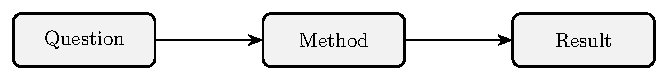
\includegraphics[width=\linewidth]{figures/example-diagram.pdf}
      \par\smallskip
      {\tiny 图注：替换为实际图形。}
  \end{columns}
\end{frame}

\begin{frame}{三栏等宽}
  \begin{columns}[T]
    \column{0.33\textwidth}
      \centering
      \textbf{阶段一}\\[6pt]
      描述第一阶段的核心特征或数据。
    \column{0.33\textwidth}
      \centering
      \textbf{阶段二}\\[6pt]
      描述第二阶段的核心特征或数据。
    \column{0.34\textwidth}
      \centering
      \textbf{阶段三}\\[6pt]
      描述第三阶段的核心特征或数据。
  \end{columns}
\end{frame}

% ------------------------------------------------------------------
\subsection{块与定理 / Blocks \& Theorems}
% ------------------------------------------------------------------

\begin{frame}{三种标准块}
  \begin{block}{标准块 (block)}
    用于关键事实、定义、或中性信息。
  \end{block}
  \begin{alertblock}{警示块 (alertblock)}
    用于警告、重要假设、或关键局限性。
  \end{alertblock}
  \begin{exampleblock}{示例块 (exampleblock)}
    用于数值例子、实证事实、或直觉说明。
  \end{exampleblock}
\end{frame}

\begin{frame}{定理与推论}
  \begin{theorem}[包络定理]
    设 $V(\theta) = \max_x f(x, \theta)$，则
    $\dfrac{dV}{d\theta} = \dfrac{\partial f}{\partial \theta}\big|_{x=x^*(\theta)}$。
  \end{theorem}
  \begin{corollary}
    在可微条件下，值函数关于参数的单调性由 $\partial f/\partial\theta$ 的符号决定。
  \end{corollary}
\end{frame}

\begin{frame}{定义与引理}
  \begin{definition}[纳什均衡]
    策略组合 $\sigma^*$ 是纳什均衡，当且仅当对任意参与人 $i$，
    在其他人策略不变的情况下，$i$ 无法通过单边偏离获益。
  \end{definition}
  \begin{lemma}
    任何有限博弈在混合策略意义下至少存在一个纳什均衡。
  \end{lemma}
\end{frame}

\begin{frame}{证明框架}
  \begin{proof}
    设 $x^* \notin \arg\max f(x)$，则存在 $x'$ 使得 $f(x') > f(x^*)$，
    与 $x^*$ 的最优性矛盾。故 $x^*$ 确为最大值点。
  \end{proof}
  \medskip
  \begin{exampleblock}{规范说明}
    Beamer 自动在 proof 结尾添加 $\square$，无需手动输入。
  \end{exampleblock}
\end{frame}

% ------------------------------------------------------------------
\subsection{数学公式 / Math}
% ------------------------------------------------------------------

\begin{frame}{行内与独行公式}
  行内公式：$\hat{\beta} = (X^\top X)^{-1} X^\top y$，
  或 $\text{plim}\,\hat{\beta} = \beta + (X^\top X/n)^{-1}(X^\top \varepsilon/n)$。

  \[
    \sigma^2 = \frac{1}{n}\sum_{i=1}^{n}(x_i - \bar{x})^2, \qquad
    \bar{x} = \frac{1}{n}\sum_{i=1}^{n} x_i.
  \]
\end{frame}

\begin{frame}{Align 带编号}
  \begin{align}
    \ell(\beta) &= \sum_{i=1}^{n}
      \bigl[y_i \log p_i + (1-y_i)\log(1-p_i)\bigr], \label{eq:loglik} \\
    \frac{\partial \ell}{\partial \beta} &= X^\top(y - p) = 0. \label{eq:foc}
  \end{align}
  式 \eqref{eq:loglik} 为对数似然；式 \eqref{eq:foc} 为一阶条件。
\end{frame}

\begin{frame}{矩阵}
  \[
    A = \begin{pmatrix} a_{11} & a_{12} \\ a_{21} & a_{22} \end{pmatrix}, \qquad
    B = \begin{bmatrix} 1 & 0 & 0 \\ 0 & 1 & 0 \\ 0 & 0 & 1 \end{bmatrix}, \qquad
    \det(A) = a_{11}a_{22} - a_{12}a_{21}.
  \]
\end{frame}

\begin{frame}{分段函数与 Cases}
  \[
    f(x) = \begin{cases}
      \alpha + \beta x   & \text{若 } x \geq \bar{x}, \\[4pt]
      \gamma + \delta x  & \text{若 } x < \bar{x}.
    \end{cases}
  \]
  \medskip
  注：用 \texttt{\\[4pt]} 在 cases 各行之间增加垂直间距。
\end{frame}

\begin{frame}{优化问题}
  \[
    \max_{\{c_t,\,k_{t+1}\}_{t=0}^{\infty}}
    \sum_{t=0}^{\infty} \beta^t u(c_t)
  \]
  \[
    \text{s.t.} \quad c_t + k_{t+1} = A k_t^\alpha, \quad
    c_t \geq 0, \quad k_0 \text{ 给定}.
  \]
  \begin{itemize}
    \item $\beta \in (0,1)$：折现因子；\quad $\alpha \in (0,1)$：资本份额。
    \item 贝尔曼方程：$V(k) = \max_{k'} \bigl\{u(Ak^\alpha - k') + \beta V(k')\bigr\}$。
  \end{itemize}
\end{frame}

% ------------------------------------------------------------------
\subsection{叠加动画 / Overlays \& Animations}
% ------------------------------------------------------------------

\begin{frame}{逐步显示：\texttt{\textbackslash pause}}
  \begin{itemize}
    \item 第一条：出现在第 1 页。
    \pause
    \item 第二条：出现在第 2 页。
    \pause
    \item 第三条：出现在第 3 页。
  \end{itemize}
  \pause
  \begin{exampleblock}{小结（第 4 页）}
    结合具体内容决定在何处插入 \texttt{\textbackslash pause}。
  \end{exampleblock}
\end{frame}

\begin{frame}{条件替换：\texttt{\textbackslash only}}
  \only<1>{
    \begin{block}{步骤 1 — 建模}
      定义参与人、策略空间和支付函数。
    \end{block}
  }
  \only<2>{
    \begin{block}{步骤 2 — 求解}
      对每位参与人求最优反应函数，联立求解。
    \end{block}
  }
  \only<3>{
    \begin{block}{步骤 3 — 解读}
      分析均衡的经济含义与福利性质。
    \end{block}
  }
  \vspace{0.5cm}
  \centering\footnotesize
  [\only<1>{第 1/3 页}\only<2>{第 2/3 页}\only<3>{第 3/3 页}]
\end{frame}

\begin{frame}{关键词逐步高亮：\texttt{\textbackslash alert<>}}
  估计策略分三步：
  \begin{itemize}
    \item<1-> \alert<1>{识别}：利用准随机变异剥离内生性。
    \item<2-> \alert<2>{估计}：对简约式做 OLS，获得降维方程。
    \item<3-> \alert<3>{推断}：使用聚类稳健标准误进行显著性检验。
  \end{itemize}
\end{frame}

\begin{frame}{未来条目置灰：\texttt{transparent}}
  {%  使用大括号将效果限制在本帧
    \setbeamercovered{transparent}
    \begin{itemize}
      \item<1-> 条目一（第 1 页完全可见，后续置灰）
      \item<2-> 条目二（第 2 页完全可见）
      \item<3-> 条目三（第 3 页完全可见）
    \end{itemize}
  }
\end{frame}

% ------------------------------------------------------------------
\subsection{图形与 TikZ / Figures \& TikZ}
% ------------------------------------------------------------------

\begin{frame}{并排双图（minipage）}
  \begin{columns}[c]
    \column{0.48\textwidth}
      \begin{figure}
        \centering
        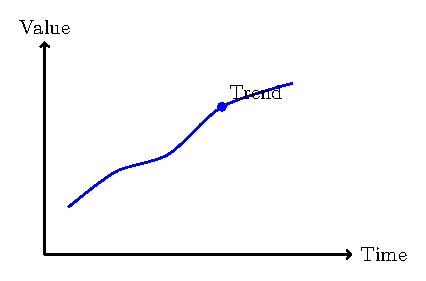
\includegraphics[width=\linewidth,height=0.48\textheight,
                         keepaspectratio]{figures/example-chart.pdf}
        \caption{面板 A：处理组}
      \end{figure}
    \column{0.48\textwidth}
      \begin{figure}
        \centering
        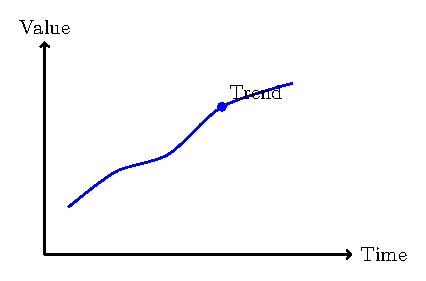
\includegraphics[width=\linewidth,height=0.48\textheight,
                         keepaspectratio]{figures/example-chart.pdf}
        \caption{面板 B：对照组}
      \end{figure}
  \end{columns}
\end{frame}

\begin{frame}{TikZ — 因果有向图 (DAG)}
  \centering
  \begin{tikzpicture}[
      node distance=1.8cm and 2.6cm,
      box/.style={draw, rounded corners=4pt,
                  minimum width=1.9cm, minimum height=0.65cm,
                  font=\small, fill=white},
      >=Stealth, thick
    ]
    \node[box] (Z) {工具变量 $Z$};
    \node[box, right=of Z] (X) {处理变量 $X$};
    \node[box, right=of X] (Y) {结果变量 $Y$};
    \node[box, dashed, above right=0.55cm and 0.9cm of X]
          (U) {不可观测 $U$};
    \draw[->] (Z) -- (X);
    \draw[->] (X) -- (Y);
    \draw[->, dashed, gray] (U) -- (X);
    \draw[->, dashed, gray] (U) -- (Y);
    \draw[->, red!70!black, bend right=18]
          node[below, font=\scriptsize, midway]{排除限制} (Z.south) to (Y.south);
    % 注：上面的 bend right 箭头演示"违反排除限制"的情形，
    %     实际使用时可删去。
  \end{tikzpicture}
  \par\smallskip
  {\footnotesize 虚线 = 不可观测路径；红色弯箭头 = 违反排除限制（示意）。}
\end{frame}

\begin{frame}{TikZ — 流程图}
  \centering
  \begin{tikzpicture}[
      node distance=0.75cm,
      box/.style={draw, rounded corners=3pt,
                  minimum width=3.4cm, minimum height=0.58cm,
                  align=center, font=\small, fill=blue!5},
      dec/.style={draw, diamond, aspect=2.6,
                  minimum width=2.8cm, font=\small, fill=orange!10},
      >=Stealth, thick
    ]
    \node[box]  (data)  {原始数据};
    \node[box, below=of data]  (clean) {清洗与预处理};
    \node[dec, below=of clean] (valid) {通过质检？};
    \node[box, below=of valid] (est)   {模型估计};
    \node[box, below=of est]   (rep)   {报告结果};

    \draw[->] (data)  -- (clean);
    \draw[->] (clean) -- (valid);
    \draw[->] (valid) -- node[right, font=\scriptsize]{是} (est);
    \draw[->] (valid.west) -- ++(-1.3,0)
              |- node[left, font=\scriptsize, pos=0.22]{否} (clean.west);
    \draw[->] (est)   -- (rep);
  \end{tikzpicture}
\end{frame}
\begin{frame}{TikZ — 水平时间轴}
  \centering
  \begin{tikzpicture}[>=Stealth, thick, font=\small]
    
    % 1. 调整背景框的深度（下移至 -0.85）
    \fill[blue!15, rounded corners=2pt] (2.2,-0.55) rectangle (6.8, 0.05);
    % 2. 将“样本期间”文字下移（Y坐标从 -0.35 改为 -0.65），避开“2008”
    \node[font=\scriptsize, text=blue!60!black] at (4.5,-0.65) {样本期间};

    % 3. 绘制主时间轴和年份刻度
    \draw[->] (-0.3,0) -- (9.2,0) node[right] {年份};
    \foreach \x/\yr in {0.5/1990, 2.5/2000, 4.5/2008, 6.5/2015, 8.5/2023}{
      \draw (\x, 0.12) -- (\x,-0.12) node[below] {\yr};
    }
    
    % 4. 事件标注（上方）
    \node[above, align=center, font=\scriptsize] at (0.5, 0.22) {改革 A};
    \node[above, align=center, font=\scriptsize] at (2.5, 0.22) {改革 B};
    \node[above, align=center, font=\scriptsize, text=red!70!black]
          at (4.5, 0.22) {金融危机};
    \node[above, align=center, font=\scriptsize] at (6.5, 0.22) {政策 C};
    \node[above, align=center, font=\scriptsize] at (8.5, 0.22) {今日};
    
    % 5. 当前位置标记
    \draw[red!70!black, thick] (8.5,0.35) -- (8.5,-0.12);
    
  \end{tikzpicture}
\end{frame}
% ------------------------------------------------------------------
\subsection{表格样例 / Tables}
% ------------------------------------------------------------------

\begin{frame}{描述性统计}
  \begin{table}
  \centering
  \caption{描述性统计（Summary Statistics）}
  {\small
  \begin{tabular}{lrrrr}
    \toprule
    变量 & 均值 & 标准差 & 最小值 & 最大值 \\
    \midrule
    人均 GDP（美元）       & 12{,}450 & 3{,}821 & 5{,}200  & 24{,}100 \\
    失业率（\%）           &     6.2  &    2.1  &     1.8  &     14.3 \\
    通货膨胀率（\%）       &     3.4  &    1.9  &  $-$0.5  &     11.2 \\
    贸易开放度             &    0.68  &   0.22  &    0.12  &      1.45 \\
    城镇化率（\%）         &    56.3  &   14.7  &    22.0  &     89.4 \\
    人力资本指数           &     2.8  &    0.6  &     1.5  &      4.1 \\
    \midrule
    样本量 $N$             & \multicolumn{4}{c}{1{,}200} \\
    \bottomrule
  \end{tabular}}
  \par\smallskip
  \raggedright
  {\footnotesize \textit{注}：年度面板数据，2000--2020 年。
  样本限于人口超过 100 万的国家。}
\end{table}

\end{frame}

\begin{frame}{多列回归比较}
  \begin{table}
  \centering
  \caption{回归结果：四种设定（Regression Results）}
  {\scriptsize
  \begin{tabular}{lcccc}
    \toprule
    & (1) OLS & (2) OLS & (3) IV & (4) IV \\
    & 基准    & +控制变量 & 基准  & +控制变量 \\
    \midrule
    处理变量          & 0.125*** & 0.098**  & 0.187*** & 0.142** \\
                      & (0.031)  & (0.040)  & (0.055)  & (0.063) \\[4pt]
    对数收入          &          & 0.234*** &          & 0.211*** \\
                      &          & (0.022)  &          & (0.025) \\[4pt]
    教育年限          &          & 0.044*   &          & 0.039*  \\
                      &          & (0.024)  &          & (0.022) \\
    \midrule
    控制变量          & 否  & 是  & 否  & 是  \\
    固定效应          & 否  & 是  & 否  & 是  \\
    $N$               & 1{,}200 & 1{,}200 & 1{,}200 & 1{,}200 \\
    $R^2$             & 0.18 & 0.34 & --- & --- \\
    F 统计（弱工具）  &      &      & 18.7 & 21.3 \\
    \bottomrule
    \multicolumn{5}{l}{%
      \scriptsize
      *** $p<0.01$，** $p<0.05$，* $p<0.1$。括号内为聚类稳健标准误。}
  \end{tabular}}
\end{table}

\end{frame}

\begin{frame}[shrink=20]{双面板（Panel A / B）异质性}
  \begin{table}
  \centering
  \caption{异质性分析：双面板（Two-Panel Heterogeneity）}
  {\footnotesize
  \begin{tabular}{lcc}
    \toprule
    & (1) 低收入组 & (2) 高收入组 \\
    \midrule
    \multicolumn{3}{l}{\textit{面板 A：城市样本}} \\
    \midrule
    处理效应   & 0.142**  & 0.098*   \\
               & (0.058)  & (0.052)  \\
    控制变量   & 是       & 是       \\
    $N$        & 600      & 600      \\
    \midrule
    \multicolumn{3}{l}{\textit{面板 B：农村样本}} \\
    \midrule
    处理效应   & 0.072    & 0.031    \\
               & (0.074)  & (0.069)  \\
    控制变量   & 是       & 是       \\
    $N$        & 400      & 400      \\
    \midrule
    \multicolumn{3}{l}{\textit{面板差异（A $-$ B）}} \\
    \midrule
    差值       & 0.070    & 0.067    \\
    $p$ 值     & 0.043    & 0.061    \\
    \bottomrule
    \multicolumn{3}{l}{%
      \footnotesize ** $p<0.05$，* $p<0.1$。括号内为聚类稳健标准误。}
  \end{tabular}}
\end{table}

\end{frame}

\begin{frame}{行高亮表格（colortbl）}
  % 需要在 main.tex 中加载 \usepackage{colortbl}
  \begin{table}
    \centering
    \caption{带高亮行的表格示例}
    \begin{tabular}{lcc}
      \toprule
      变量 & 处理组 & 对照组 \\
      \midrule
      \rowcolor{yellow!30}
      GDP 增速 (\%) & 6.8 & 3.2 \\
      失业率 (\%)   & 4.1 & 7.6 \\
      \rowcolor{yellow!30}
      通货膨胀 (\%) & 2.3 & 4.8 \\
      贸易开放度    & 0.72 & 0.51 \\
      \bottomrule
    \end{tabular}
  \end{table}
  {\footnotesize \textit{注}：黄色行为核心关注变量。}
\end{frame}

% ------------------------------------------------------------------
\subsection{代码与逐字排版 / Code \& Verbatim}
% ------------------------------------------------------------------

\begin{frame}[fragile]{Python 代码（listings）}
  % 需要在 main.tex 中加载 \usepackage{listings} 并配置 \lstset
  \begin{lstlisting}[language=Python, caption={OLS 估计量（NumPy 实现）}]
import numpy as np

def ols(X, y):
    """返回 OLS 系数向量 beta_hat."""
    return np.linalg.solve(X.T @ X, X.T @ y)

# 生成模拟数据
rng  = np.random.default_rng(42)
X    = np.column_stack([np.ones(200), rng.standard_normal((200, 2))])
beta = np.array([1.0, 2.0, -0.5])
y    = X @ beta + rng.standard_normal(200)

print(ols(X, y))   # 应接近 [1, 2, -0.5]
  \end{lstlisting}
\end{frame}

\begin{frame}[fragile]{LaTeX 代码排版（lstlisting）}
  % ⚠ Beamer 限制：[fragile] 帧的内容（含 \input 子文件）里
  %   不能出现字面的 \end{frame}，否则 Beamer 预扫描会误判帧结束。
  %   解决方法：只展示帧内部代码，外层 \begin/\end{frame} 用文字说明。
  \begin{lstlisting}[language=TeX, caption={帧内叠加动画（内部代码）}]
% 以下内容放在 frame 环境内部（外层为 \begin{frame}...\end{...} 结构）：
\begin{itemize}
  \item<1-> \alert<1>{Step 1}: 建立模型
  \item<2-> \alert<2>{Step 2}: 求解均衡
  \item<3-> \alert<3>{Step 3}: 实证检验
\end{itemize}
\setbeamercovered{transparent}  % 未到场条目置灰
  \end{lstlisting}
  {\footnotesize\textit{注}：若需在代码块中展示完整帧结构（含 \texttt{\textbackslash end\{frame\}}），
  可将代码存入独立 \texttt{.tex} 文件后用 \texttt{\textbackslash lstinputlisting} 引入。}
\end{frame}

% ------------------------------------------------------------------
\subsection{特殊幻灯片与导航 / Special Slides \& Navigation}
% ------------------------------------------------------------------

\begin{frame}{章节过渡页}
  \vspace*{\fill}
  \begin{center}
    {\Large \textbf{第~\Roman{section}~部分}}\\[0.7em]
    {\large \insertsectionhead}\\[1.2em]
    {\normalsize 一句话预告本节核心内容。}
  \end{center}
  \vspace*{\fill}
\end{frame}

\begin{frame}{进度路线图（手动高亮当前节）}
  \begin{enumerate}
    \item[\checkmark] 引言
    \item[\checkmark] 背景与文献
    \item[\textbf{3.}] \textbf{模型} \quad \textcolor{blue}{$\leftarrow$ 当前}
    \item[4.] \textcolor{gray}{实证分析}
    \item[5.] \textcolor{gray}{结论}
  \end{enumerate}
\end{frame}

\begin{frame}{两箱对比（alertblock vs exampleblock）}
  \begin{columns}[T]
    \column{0.48\textwidth}
      \begin{alertblock}{无干预（基准）}
        \begin{itemize}
          \item 产出增速：低
          \item 失业率：高
          \item 社会福利：$W_0$
        \end{itemize}
      \end{alertblock}
    \column{0.48\textwidth}
      \begin{exampleblock}{有干预（反事实）}
        \begin{itemize}
          \item 产出增速：高
          \item 失业率：低
          \item 社会福利：$W_1 > W_0$
        \end{itemize}
      \end{exampleblock}
  \end{columns}
\end{frame}

\begin{frame}{引言页 / Pull Quote}
  \vspace*{\fill}
  \begin{center}
    \Large\itshape
    ``好的模型不求包罗万象，\\
    只求能对关键机制给出清晰预测。''
    \vspace{0.9em}

    \normalsize\upshape
    --- 示例引用，\textit{来源书目}，年份
  \end{center}
  \vspace*{\fill}
\end{frame}

% 超链接导航示例
% 用法：目标帧内加 \label{frm:target}，此处用 \hyperlink{frm:target}{按钮}
\begin{frame}{附录跳转按钮}
  正文幻灯片可加入指向附录的按钮，听众提问时快速跳转：

  \medskip
  \hyperlink{frm:robustness}{\beamergotobutton{稳健性检验}}
  \hspace{1em}
  \hyperlink{frm:derivation}{\beamergotobutton{完整推导}}
  \hspace{1em}
  \hyperlink{frm:data}{\beamergotobutton{数据说明}}

  \bigskip
  附录帧返回正文：

  \medskip
  \hyperlink{frm:main-results}{\beamerreturnbutton{返回主结果}}
  \hspace{1em}
  \hyperlink{frm:empirics}{\beamerbutton{跳至实证节}}

  \bigskip
  {\footnotesize \textit{用法}：在目标帧内加
    \texttt{\textbackslash label\{frm:robustness\}} 等标签即可激活以上按钮。}
\end{frame}


\begin{frame}
  \vspace*{\fill}
  \begin{center}
    {\Huge \textbf{谢谢聆听！}} \\[1em]
    {\large Q \& A}
  \end{center}
  \vspace*{\fill}
  
  \begin{center}
    \tiny \textcolor{gray}{
      \ccby \\ % 这里会渲染出 CC 和 BY 的官方小图标
      This work is licensed under a \href{https://creativecommons.org/licenses/by/4.0/}{Creative Commons Attribution 4.0 International License}.
    }
  \end{center}
\end{frame}

\end{document}
